\documentclass[11pt,letterpaper]{article}

% ============ DATOS DEL ESTUDIANTE ============
\newcommand{\nombreEstudiante}{Duván Felipe Baquero}
\newcommand{\codigoEstudiante}{160005002}
\newcommand{\nombreDocente}{Ángel Alfonso Cruz Roa}
% ==============================================

% Preámbulo agnóstico al motor: sirve con pdfLaTeX, XeLaTeX y LuaLaTeX.
\usepackage{iftex}
\ifPDFTeX
  \usepackage[utf8]{inputenc}
  \usepackage[T1]{fontenc}
  \usepackage{lmodern}
\else
  \usepackage{fontspec}
\fi

% babel-spanish redefine \% y rompe \,\% y el \% dentro de modo matemático.
\let\origpercent\%
\usepackage[spanish,es-tabla,es-nodecimaldot]{babel}
\AtBeginDocument{\let\%\origpercent}

\usepackage[margin=2.5cm]{geometry}
\usepackage{graphicx}
\usepackage{booktabs}
\usepackage{array}
\usepackage{longtable}
\usepackage{amsmath}
\usepackage{amssymb}
\usepackage{float}
\usepackage{xcolor}
\usepackage{fancyhdr}
\usepackage{caption}
\usepackage{subcaption}
\usepackage{enumitem}
\usepackage{microtype}
\usepackage{tocloft}
\usepackage{listings}
\usepackage[hidelinks]{hyperref}

\setlength{\cftbeforesecskip}{0.25em}\setlength{\cftbeforesubsecskip}{0em}
\renewcommand{\cftsubsecfont}{\small}\renewcommand{\cftsubsecpagefont}{\small}
\captionsetup{font=small,labelfont=bf,skip=6pt}
\setlength{\parskip}{0.35em}
\setlength{\emergencystretch}{3em}
\renewcommand{\arraystretch}{1.12}

\definecolor{fondocodigo}{RGB}{246,247,249}
\lstset{language=Python, basicstyle=\ttfamily\footnotesize, backgroundcolor=\color{fondocodigo},
  frame=single, rulecolor=\color{gray!40}, columns=fullflexible, keepspaces=true,
  showstringspaces=false, breaklines=true, commentstyle=\color{gray}, keywordstyle=\color{blue!60!black},
  xleftmargin=4pt, xrightmargin=4pt, aboveskip=6pt, belowskip=6pt}
\lstdefinestyle{salida}{language={}, backgroundcolor=\color{white}, basicstyle=\ttfamily\scriptsize,
  frame=leftline, rulecolor=\color{gray!60}}

% Capturas de AnyLogic: si el archivo existe en capturas/ se inserta; si no, queda un recuadro.
\newcommand{\captura}[3][0.9]{%
  \begin{figure}[H]\centering
  \IfFileExists{capturas/#2}{\includegraphics[width=#1\textwidth]{capturas/#2}}%
  {\fbox{\parbox[c][4.2cm][c]{#1\textwidth}{\centering\small\color{gray}Captura pendiente:\\[2pt]\texttt{capturas/\detokenize{#2}}}}}
  \caption{#3}\end{figure}}



% \input no es expandible y rompe \bottomrule dentro de tabular; se usa el primitivo
\makeatletter\newcommand{\tablain}[1]{\@@input #1 }\makeatother

\pagestyle{fancy}
\fancyhf{}
\lhead{\small Universidad de los Llanos}
\rhead{\small Simulación Computacional --- Laboratorio 4}
\rfoot{\small\thepage}
\renewcommand{\headrulewidth}{0.4pt}

\begin{document}

% =====================================================
% PORTADA
% =====================================================
\begin{titlepage}
\thispagestyle{empty}
\centering
\vspace*{\fill}

{\large \textsc{Universidad de los Llanos}}\\[0.2cm]
{\normalsize Facultad de Ciencias Básicas e Ingeniería}\\
{\normalsize Programa de Ingeniería de Sistemas}\\[1.6cm]

\rule{\textwidth}{0.8pt}\\[0.5cm]
{\LARGE \textbf{Simulación de eventos discretos}}\\[0.35cm]
{\large Línea de espera G/G/1, red de colas, inventario probabilístico,\\
SimPy y AnyLogic}\\[0.5cm]
\rule{\textwidth}{0.8pt}\\[1.6cm]

{\normalsize Informe del Laboratorio 4}\\
{\normalsize (guía FO-DOC-112, Práctica N.\textsuperscript{o}\,03)}\\
{\normalsize Curso: Simulación Computacional}\\[1.4cm]

{\normalsize Presentado por:}\\[0.15cm]
{\large \nombreEstudiante}\\
{\normalsize Código: \codigoEstudiante}\\[1.2cm]

{\normalsize Docente:}\\[0.15cm]
{\large \nombreDocente}\\[1.6cm]

{\normalsize Villavicencio, Meta \\ \today}

\vspace*{\fill}
\end{titlepage}

\newpage
\tableofcontents
\newpage

% =====================================================
\section{Objetivos}
% =====================================================

Estos son los objetivos que trae la guía de laboratorio:

\begin{itemize}[itemsep=2pt]
    \item Introducir al paradigma de simulación de eventos discretos por medio de sus elementos, diseño, metodología de modelado e implementación.
    \item Apropiar la metodología de modelado e implementación de simulación de eventos discretos a partir de dos casos de uso: un sistema de línea de espera con un servidor y una red de colas.
    \item Implementar la metodología de modelado y simulación de eventos discretos en un caso de estudio de un modelo de inventario probabilístico.
    \item Implementar casos de estudio de simulación de eventos discretos en frameworks o softwares de simulación para eventos discretos como SimPy y AnyLogic.
\end{itemize}

% =====================================================
\section{Consulta previa}
% =====================================================

\subsection{¿En qué consiste el paradigma de simulación de eventos discretos?}

En modelar un sistema cuyo estado solo cambia en instantes puntuales, llamados eventos o sucesos, y
suponer que entre dos eventos seguidos no pasa nada relevante. En una fila de banco, por ejemplo, el número
de clientes solo cambia cuando alguien llega o cuando alguien termina de ser atendido. Por eso el reloj de la
simulación no avanza de a poco, sino que salta de un evento al siguiente (simulación asíncrona). En cada salto
se actualizan el estado y los contadores y se programan los eventos futuros que el evento actual genera. Esto
lo diferencia de la simulación continua, donde el estado cambia todo el tiempo y se describe con ecuaciones
diferenciales, y de la simulación síncrona, que avanza en pasos fijos $\Delta t$ aunque no ocurra nada.

\subsection{¿Cuáles son los elementos y la metodología de modelado de la simulación de eventos discretos?}

Según \cite{rios08}, los elementos básicos son las variables y los sucesos. Las variables son de tres tipos:

\begin{itemize}[itemsep=1pt]
\item la \textbf{variable de tiempo} $t$, que lleva el tiempo simulado transcurrido;
\item las \textbf{variables de estado}, que describen el sistema en el instante $t$ (número de clientes en
cola, nivel del inventario);
\item los \textbf{contadores}, que acumulan lo que ha pasado hasta $t$ (llegadas, salidas, costos) y con los
que al final se calculan las medidas de desempeño.
\end{itemize}

A esto se suma una \textbf{lista de sucesos}, que en los ejemplos del curso es la estructura
\texttt{TSuc}: guarda el instante de cada suceso pendiente y un valor muy grande $M$ cuando no hay ninguno.
El programa principal repite siempre lo mismo: busca en la lista el suceso más próximo, avanza el reloj hasta
él y ejecuta la rutina de ese tipo de suceso, que cambia el estado, actualiza contadores y programa sucesos
nuevos. Cuando la lista queda vacía se calculan las salidas.

La metodología de modelado es iterativa: se define el problema y las fronteras del sistema, se formulan
hipótesis, se construye un modelo básico y luego uno simplificado que sea tratable, se implementa, se
verifica (que el programa haga lo que el modelo dice), se valida (que el modelo represente el sistema real) y
se experimenta con él. Si una etapa no es satisfactoria se vuelve a la anterior. Como la salida es aleatoria,
la experimentación exige hacer varias réplicas y resumirlas con medias, desviaciones e intervalos de
confianza.

\subsection{¿En qué consiste un sistema de cola simple?}

En un sistema con una sola fuente de clientes, una sola cola y un solo servidor. Los clientes llegan según un
proceso aleatorio; si el servidor está libre se atienden de inmediato y si no, esperan en la cola, casi siempre
en orden de llegada (FIFO). Se describe con la notación de Kendall: G/G/1 significa tiempos entre llegadas y de
servicio con distribuciones generales y un servidor, y M/M/1 el caso particular en que ambos son exponenciales.
El parámetro que más pesa es la intensidad de tráfico $\rho = \lambda/\mu$, el cociente entre la tasa de
llegadas y la de servicio. Si $\rho < 1$ el sistema alcanza un régimen estable, y si $\rho \ge 1$ la cola crece
sin límite. Las medidas usuales son el tiempo medio en el sistema y en la cola, el número medio de clientes y
la utilización del servidor.

\subsection{¿En qué consiste una red de colas?}

En un conjunto de nodos de servicio, cada uno con su cola, conectados de forma que la salida de uno es la
entrada de otro. Un cliente recorre varios nodos según reglas de ruteo, que pueden ser fijas o
probabilísticas. En la red del numeral 5.2, por ejemplo, el 40\,\% de los vehículos pasa de la ventanilla a una
nave auxiliar y el 60\,\% va directo a la nave principal. Las redes pueden ser abiertas (los clientes entran y
salen, como en ese caso) o cerradas (circula siempre la misma población). Algunos casos tienen solución
analítica, como las redes de Jackson con servicios exponenciales, pero en cuanto aparecen servicios normales o
tiempos que dependen del estado de la cola, como en la ITV, la simulación es la única herramienta práctica.

\subsection{¿En qué consiste un inventario probabilístico?}

En un sistema de almacenamiento en el que la demanda, los tiempos de entrega o ambos son aleatorios. La
empresa tiene que decidir cuándo pedir y cuánto pedir (su política de inventario) para equilibrar tres costos
que se contraponen: el de almacenar mucho, el de pedir seguido y el de quedarse sin producto y perder ventas.
En el modelo de \cite{rios08} los clientes llegan como un proceso de Poisson, cada uno pide una cantidad
aleatoria y la política es de tipo $(p, P)$: cuando el inventario baja de $p$ y no hay pedido pendiente, se pide
lo necesario para volver a $P$, y el pedido tarda $L$ en llegar. Como no hay fórmulas cerradas para este caso,
el beneficio, la fracción de clientes satisfechos y el tiempo con inventario en cero se estiman simulando.

\subsection{¿Qué es el framework SimPy para simulación de eventos discretos?}

SimPy es una librería de Python, de código abierto, para simulación de eventos discretos basada en
procesos. Los procesos (clientes, máquinas, vehículos) se escriben como funciones generadoras de Python, y
cada \texttt{yield} de un evento suspende el proceso hasta que ese evento ocurra. Un \texttt{Environment}
maneja el reloj y la cola de eventos, y hay recursos compartidos ya hechos: \texttt{Resource} (servidores con
cola), \texttt{Container} (cantidades continuas o a granel) y \texttt{Store} (objetos individuales), con
variantes con prioridad y con desplazamiento. La diferencia con la implementación de los numerales 5.1 a 5.3 es
que en SimPy no se programa la lista de sucesos: se describe lo que hace cada entidad y la librería decide
en qué orden se ejecuta todo.

\subsection{¿Cómo usar el software de simulación AnyLogic para simulación de eventos discretos?}

AnyLogic es un entorno gráfico de simulación que combina eventos discretos, sistemas dinámicos y modelado
basado en agentes. Para eventos discretos se usa sobre todo la \emph{Process Modeling Library}: el modelo se
arma como un diagrama de flujo con bloques que se arrastran desde la paleta y se conectan
(\texttt{Source} crea las entidades, \texttt{Queue} las pone en cola, \texttt{Delay} y \texttt{Service} las
retienen un tiempo, \texttt{SelectOutput} las enruta, \texttt{ResourcePool} define recursos y \texttt{Sink}
las elimina). Cada bloque se configura en su panel de propiedades con distribuciones como
\texttt{triangular()} o \texttt{exponential()}. Encima del diagrama se dibuja el espacio (nodos, rutas,
bandas transportadoras) y se añade animación 2D o 3D. Para casos especializados están la \emph{Pedestrian
Library}, la \emph{Road Traffic Library}, la \emph{Material Handling Library} y la \emph{Fluid Library}. Al
ejecutar, los bloques recogen estadísticas por su cuenta (utilización, tamaño de cola) que se pueden llevar a
gráficas. La versión gratuita PLE (\emph{Personal Learning Edition}) es la que se usó en el numeral 5.5.

% =====================================================
\section{Metodología y herramientas}
% =====================================================

Los numerales 5.1 a 5.4 se desarrollaron en cuatro cuadernos de Jupyter en Python, ejecutados de principio a fin
y adjuntos a este informe:

\begin{center}
\begin{tabular}{@{}ll@{}}
\toprule
Numeral & Archivo \\
\midrule
5.1 Línea de espera G/G/1 & \texttt{Lab4\_5.1\_GG1\_\codigoEstudiante.ipynb} \\
5.2 Red de colas & \texttt{Lab4\_5.2\_RedColas\_\codigoEstudiante.ipynb} \\
5.3 Inventario probabilístico & \texttt{Lab4\_5.3\_Inventario\_\codigoEstudiante.ipynb} \\
5.4 SimPy & \texttt{Lab4\_5.4\_SimPy\_\codigoEstudiante.ipynb} \\
\bottomrule
\end{tabular}
\end{center}

Se usaron \texttt{numpy}, \texttt{pandas}, \texttt{matplotlib}, \texttt{scipy} y \texttt{simpy}~4.1.2, y los
cuadernos corren en Google Colab sin instalar nada más que SimPy. Todas las semillas están fijas, así que cada
ejecución reproduce exactamente las tablas y figuras de este informe. El numeral 5.5 se desarrolló en AnyLogic
8.9 PLE; los modelos \texttt{.alp} se entregan en la carpeta \texttt{Modelos\_AnyLogic}.

Los numerales 5.1 y 5.2 parten de copias de los cuadernos de ejemplo del curso y conservan su estructura:
variables globales, una rutina por tipo de suceso y un bucle principal que recorre la lista \texttt{TSuc}. Al
correrlos aparecieron dos errores de cálculo en los ejemplos, uno en cada cuaderno, que se corrigieron y se
documentan en su sección. El numeral 5.3 se escribió desde cero siguiendo el pseudocódigo de la sección 5.6 de
\cite{rios08}, con la misma estructura de los otros dos.

% =====================================================
\section{Numeral 5.1: sistema de línea de espera con un servidor}
% =====================================================

\subsection{El modelo y los cambios hechos al ejemplo}

El cuaderno de ejemplo implementa la cola G/G/1 de la sección 5.5.1 de \cite{rios08}. Hay dos sucesos, la
llegada de un cliente (\texttt{tLL}) y la salida del servidor (\texttt{tS}). El estado es el número de
clientes $n$ en el sistema. Se aceptan llegadas hasta el instante $T$ y después el servidor sigue trabajando
hasta vaciar la cola. Los números uniformes salen de dos generadores congruenciales mixtos, uno para las
llegadas y otro para los servicios.

Sobre ese código se hicieron cuatro cambios:

\begin{enumerate}[itemsep=2pt]
\item \texttt{GenerarX} y \texttt{GenerarY} toman los parámetros del escenario en lugar de tener
\texttt{vlambda = 5} fijo. Se conservó la convención del ejemplo, en la que $\lambda$ es una tasa:
$X = -\ln(1-U)/\lambda$, con media $1/\lambda$.
\item Para el escenario B se agregó un generador normal por el método polar, que toma sus uniformes de
\texttt{gencongru2}, y el truncamiento en cero que pide la nota de la guía. Antes de usarlo se probaron 20\,000
valores: media 0,013, desviación 1,002 y prueba de Kolmogorov--Smirnov con $p = 0{,}17$.
\item El bucle principal quedó dentro de una función \texttt{simular()} para poder repetirlo, y los
generadores se reinician al comenzar cada escenario. Así la corrida 1 es reproducible y las corridas 2 a 10
siguen la secuencia.
\item \textbf{Corrección de los tiempos medios.} Las listas \texttt{LL}, \texttt{S} y \texttt{Serv} empiezan
con un valor ficticio $0$ en la posición 0, de modo que el cliente $i$ queda en la posición $i$. El ejemplo
sumaba las posiciones $0, \dots, \texttt{NLL}-1$, así que incluía el cero ficticio y dejaba por fuera al
último cliente. Ahora se suman las posiciones $1, \dots, \texttt{NLL}$. En la primera corrida del escenario A
el tiempo medio en el sistema pasa de 13,0940 con el cálculo original a 13,2105 con el corregido.
\end{enumerate}

\subsection{Escenario A}

$T = 40$, tiempos entre llegadas exponenciales con $\lambda = 5$ y tiempos de servicio exponenciales con
$\lambda = 3$. Llegan 5 clientes por unidad de tiempo y el servidor puede atender 3, así que
$\rho = 5/3 \approx 1{,}67$: el sistema es inestable.

\begin{figure}[H]
\centering
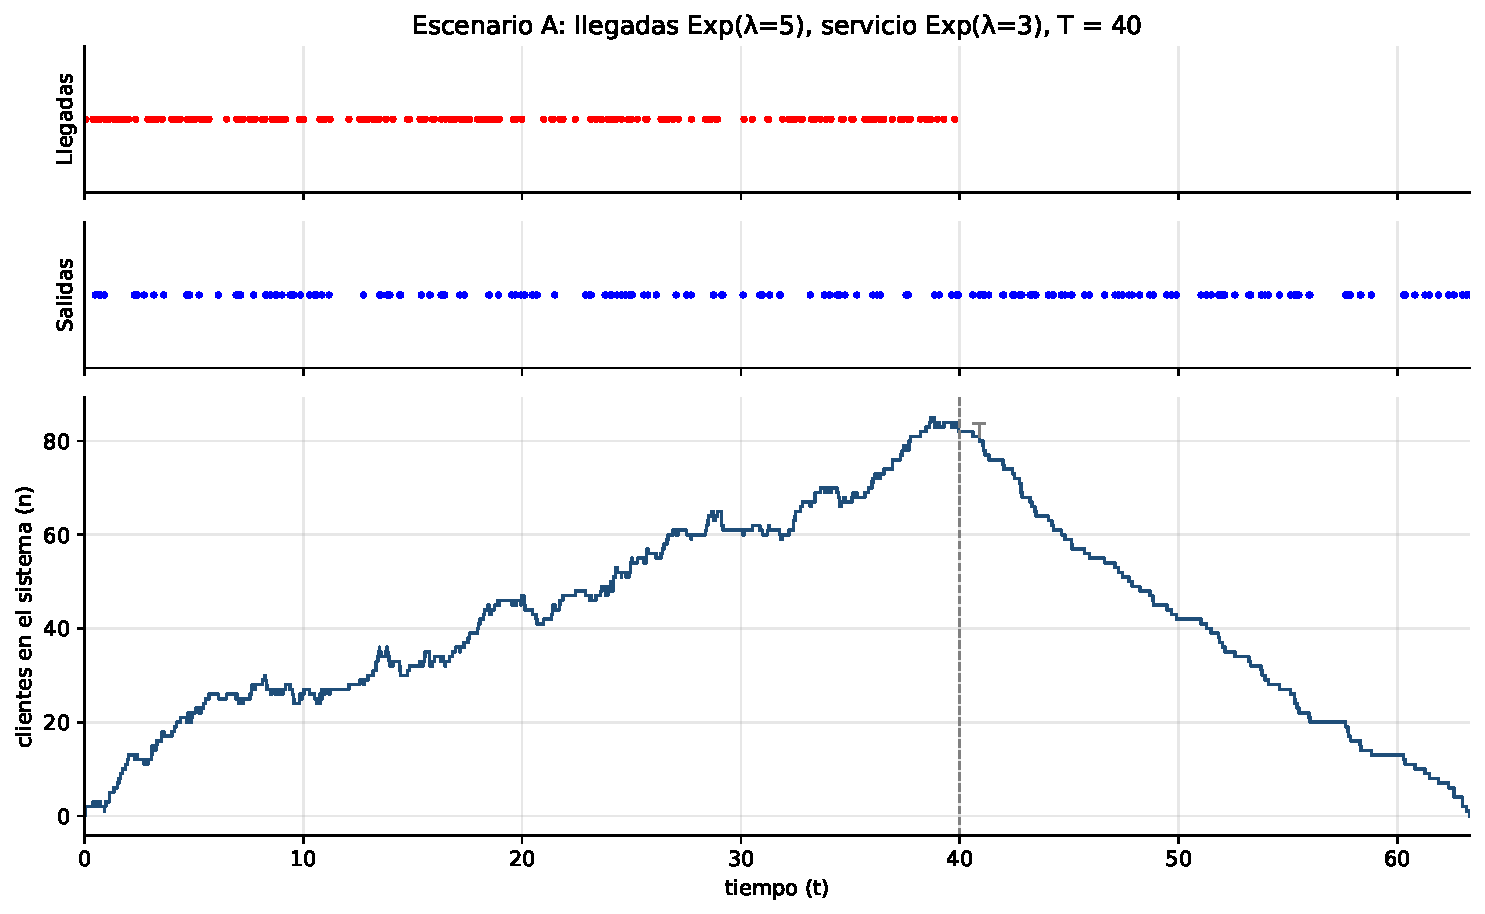
\includegraphics[width=0.86\textwidth]{figuras/51_escA.pdf}
\caption{Escenario A, primera corrida: instantes de llegada, instantes de salida y número de clientes en el
sistema. La línea punteada marca $T = 40$.}
\label{fig:51A}
\end{figure}

Respuestas con la primera corrida:

\begin{itemize}[itemsep=1pt]
\item Tiempo medio de los clientes en el sistema: 13,2105.
\item Tiempo medio de los clientes en la cola: 12,8973.
\item Tiempo transcurrido desde $T$ hasta que el último cliente abandona el sistema: 23,3130.
\item Número máximo de clientes en el sistema: 85.
\item Total de clientes que pasaron por el sistema: 202.
\end{itemize}

La figura \ref{fig:51A} muestra lo que se espera con $\rho > 1$: el número de clientes sube casi en línea recta
durante toda la ventana de llegadas, llega a 85 justo en $T$ y a partir de ahí solo baja. La diferencia entre
el tiempo en el sistema y el tiempo en cola es 0,31, muy cerca del tiempo medio de servicio de $1/3$. Un cliente
pasa casi todo su tiempo esperando.

\subsection{Escenario B}

$T = 40$, tiempos entre llegadas exponenciales con $\lambda = 1$ y tiempos de servicio normales con $\mu = 2$ y
$\sigma = 1$, truncados en cero. Ahora $\rho \approx 2$. El truncamiento casi no cambia la media, porque
$P\{Y < 0\} = \Phi(-2) \approx 2{,}3\,\%$.

\begin{figure}[H]
\centering
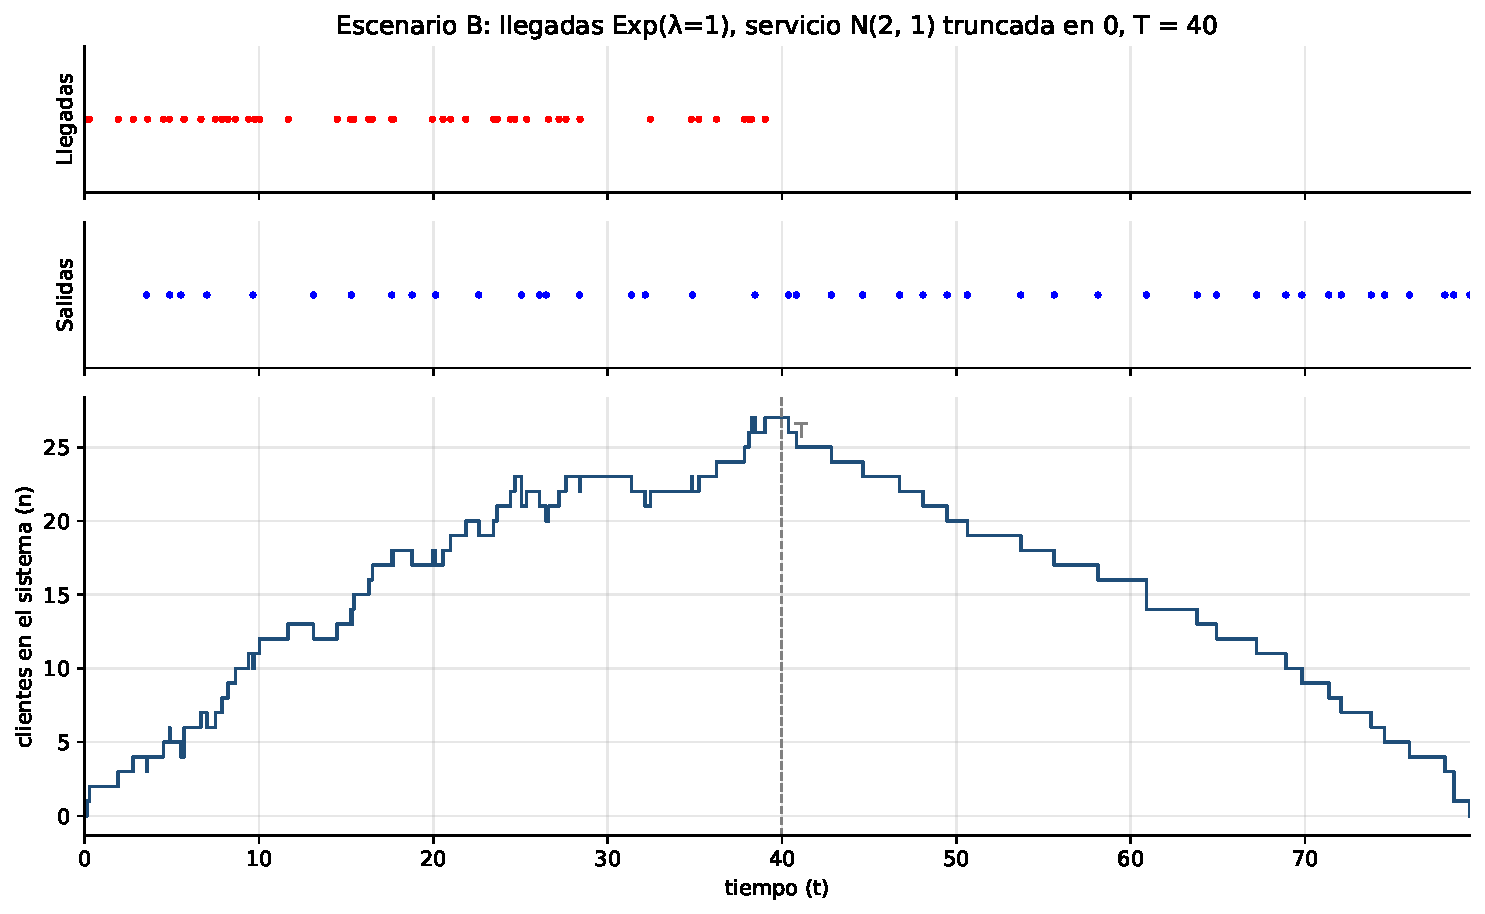
\includegraphics[width=0.86\textwidth]{figuras/51_escB.pdf}
\caption{Escenario B, primera corrida.}
\label{fig:51B}
\end{figure}

Respuestas con la primera corrida:

\begin{itemize}[itemsep=1pt]
\item Tiempo medio de los clientes en el sistema: 26,1985.
\item Tiempo medio de los clientes en la cola: 24,5107.
\item Tiempo transcurrido desde $T$ hasta que el último cliente abandona el sistema: 39,4699.
\item Número máximo de clientes en el sistema: 27.
\item Total de clientes que pasaron por el sistema: 47.
\end{itemize}

En esta corrida entraron 47 clientes, más de los 40 esperados, y la media de los servicios fue 1,69 en lugar
de 2; 3 de los 47 quedaron truncados en cero. Con 47 datos y $\sigma \approx 1$, una media de 1,69 está a unos
dos errores estándar de 2, así que es variación de la muestra y no un defecto del generador, como ya había
confirmado la prueba de los 20\,000 valores.

\subsection{Diez simulaciones por escenario}

Las tablas \ref{tab:51corrA} y \ref{tab:51corrB} tienen las diez corridas de cada escenario y la tabla
\ref{tab:51} las resume en el formato que pide la guía.

\begin{table}[H]
\centering
\caption{Escenario A: diez corridas.}
\label{tab:51corrA}
\small
\begin{tabular}{@{}crrrrr@{}}
\toprule
Corrida & T. medio sistema & T. medio cola & Desde $T$ hasta el último & Máx. clientes & Total clientes \\
\midrule
\tablain{tablas/tab51_corridasA.tex}
\bottomrule
\end{tabular}
\end{table}

\begin{table}[H]
\centering
\caption{Escenario B: diez corridas.}
\label{tab:51corrB}
\small
\begin{tabular}{@{}crrrrr@{}}
\toprule
Corrida & T. medio sistema & T. medio cola & Desde $T$ hasta el último & Máx. clientes & Total clientes \\
\midrule
\tablain{tablas/tab51_corridasB.tex}
\bottomrule
\end{tabular}
\end{table}

\begin{table}[H]
\centering
\caption{Medidas de desempeño para los escenarios A y B luego de 10 simulaciones (promedio $\pm$ desviación
estándar muestral).}
\label{tab:51}
\small
\begin{tabular}{@{}p{7.2cm}cc@{}}
\toprule
Medida de desempeño & Escenario A & Escenario B \\
\midrule
\tablain{tablas/tab51_resumen.tex}
\bottomrule
\end{tabular}
\end{table}

\begin{figure}[H]
\centering
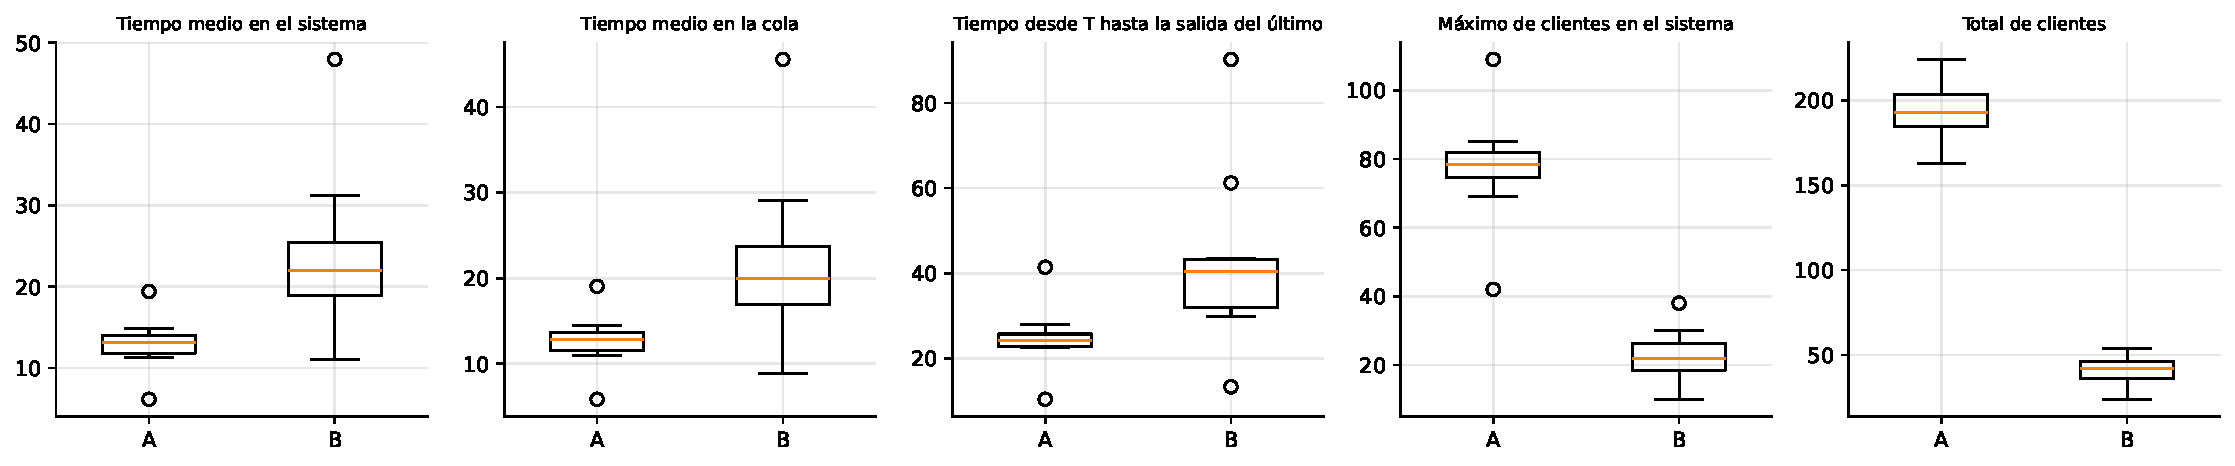
\includegraphics[width=\textwidth]{figuras/51_cajas.pdf}
\caption{Diagramas de caja de las cinco medidas en las diez corridas de cada escenario.}
\label{fig:51cajas}
\end{figure}

\subsection{¿Qué puede analizar de los resultados comparando los dos escenarios?}

Lo primero es que \textbf{los dos escenarios son inestables}: en A llegan 5 clientes por unidad de tiempo y se
atienden 3 ($\rho = 1{,}67$), y en B llega 1 y se atiende 0,5 ($\rho = 2$). No hay un régimen estable. La cola
crece mientras haya llegadas, y por eso todas las medidas dependen de $T$.

Un cálculo sencillo de ``flujo'' reproduce bastante bien la tabla \ref{tab:51}. Si la cola crece a razón de
$\lambda - \mu$ clientes por unidad de tiempo, al llegar a $T$ hay unos $(\lambda - \mu)T$ clientes en el
sistema. En A eso da $(5 - 3)\cdot 40 = 80$, frente a un máximo promedio de 77,6; vaciarlos a 3 por unidad de
tiempo toma $80/3 \approx 26{,}7$, y el tiempo después de $T$ salió 24,8. En B da $(1 - 0{,}5)\cdot 40 = 20$
frente a 22,7, y vaciarlos toma $20 \cdot 2 = 40$, frente a 42,7. Con el mismo razonamiento, un cliente que
llega en el instante $s$ encuentra unos $(\lambda - \mu)s$ clientes delante y espera cerca de $(\rho - 1)s$;
promediando sobre $[0, T]$ el tiempo en el sistema es del orden de $(\rho - 1)T/2$, es decir, 13,3 en A y 20 en
B, frente a 12,97 y 24,00 simulados.

\textbf{B es peor para el cliente aunque reciba cinco veces menos gente.} En A pasaron 194 clientes en promedio
y en B 41, pero en B cada cliente estuvo 24,0 unidades de tiempo en el sistema, casi el doble que en A (13,0), y
el último salió 42,7 unidades después de $T$, contra 24,8 en A. Lo que manda no es cuánta gente llega, sino
cuánto excede la demanda a la capacidad: en B el servidor necesitaría el doble del tiempo disponible, y en A
1,67 veces.

\textbf{B también es más variable.} El coeficiente de variación del tiempo en el sistema es 25\,\% en A
($3{,}31/12{,}97$) y 41\,\% en B ($9{,}93/24{,}00$). En la corrida 8 de B el último cliente salió 90 unidades
después de $T$ y en la corrida 9 solo 13. Con unos 40 clientes por corrida, una racha de llegadas o de servicios
largos pesa mucho; con los 200 de A esos efectos tienden a compensarse.

Por último, en los dos escenarios \textbf{la cola es casi todo el tiempo en el sistema}: la diferencia entre
ambas medidas es 0,33 en A y 2,01 en B, que son justo los tiempos medios de servicio. Más del 90\,\% del tiempo
de cada cliente se va en esperar. Mejorar un poco el servicio no alcanzaría; haría falta un segundo servidor o
limitar las llegadas hasta dejar $\rho < 1$.

% =====================================================
\section{Numeral 5.2: red de colas}
% =====================================================

\subsection{El modelo}

La red de la sección 5.5.2 de \cite{rios08} representa un centro de revisión técnico-mecánica (ITV) con tres
nodos, todos con cola FIFO de capacidad infinita:

\begin{itemize}[itemsep=1pt]
\item \textbf{N1}, ventanilla de documentación y pago, con servicio $N(\mu_1, \sigma_1)$ truncado en 0;
\item \textbf{N2}, nave auxiliar para las pruebas adicionales de los vehículos de más de 10 años (el 40\,\%),
con servicio exponencial de media $\mu_2$;
\item \textbf{N3}, nave principal por la que pasan todos, con servicio $N(\mu_{31}, \sigma_{31})$ si hay menos de 5
vehículos y $N(\mu_{32}, \sigma_{32})$ si hay 5 o más, porque los operarios se apuran cuando hay congestión.
\end{itemize}

Del nodo 1 el vehículo va a N2 con probabilidad 0,4 o directamente a N3 con probabilidad 0,6, y de N2 siempre
pasa a N3. Se aceptan llegadas hasta $T = 300$ y se sigue atendiendo hasta que sale el último.

\textbf{Convención de los parámetros.} El ejemplo genera los tiempos entre llegadas con
\texttt{np.random.exponential(L)} y los servicios de N2 con \texttt{np.random.exponential(mu2)}. NumPy
interpreta ese argumento como la media (escala), no como la tasa, y se respetó esa convención: con
$\lambda = 2$ llega en promedio un vehículo cada 2 unidades de tiempo. Leer $\lambda$ como tasa daría un
vehículo cada 0,5 unidades a una ventanilla que tarda 2,1 en promedio, y el nodo 1 recibiría cuatro veces más
de lo que puede atender.

\subsection{Correcciones al cuaderno de ejemplo}

Al revisar los resultados del primer escenario apareció una inconsistencia: por N2 pasaron 59 vehículos con un
servicio medio de 2,4, pero el número medio de vehículos en N2 salía 0,19. Por la ley de Little debía rondar
0,46. La causa es que en el ejemplo \textbf{cada rutina acumula el área $n_j(t_{suc} - t)$ solo del nodo que
ella misma modifica}, pero el reloj \texttt{t} avanza con los sucesos de todos los nodos. Si entre dos sucesos
del nodo 2 ocurre, por ejemplo, una salida del nodo 3, ese tramo se pierde para el nodo 2. El resultado es que
\texttt{n\_med\_n1}, \texttt{n\_med\_n2} y \texttt{n\_med\_n3} salen subestimados. Se corrigió con una función
\texttt{acumular\_areas()} que, al comienzo de cada suceso, suma el área de los tres nodos antes de mover el
reloj.

Había un segundo detalle: el bucle guardaba el estado $(t, n_1, n_2, n_3)$ una vez por vuelta, aunque en una
vuelta se pueden procesar hasta cuatro sucesos, y así se perdían estados intermedios y posibles máximos. Ahora el
estado se guarda después de cada suceso. Ninguno de los dos cambios toca las llamadas al generador, así que con
la misma semilla se simula exactamente la misma historia y solo cambia la forma de medir.

\begin{table}[H]
\centering
\caption{Número medio de vehículos por nodo en la primera repetición del escenario A: cálculo corregido,
verificación directa $\sum_i (S_j(i) - LL_j(i))/t$ y cálculo del ejemplo original.}
\label{tab:52verif}
\small
\begin{tabular}{@{}lccc@{}}
\toprule
Nodo & Corregido & $\sum (S - LL)/t$ & Ejemplo original \\
\midrule
N1 & 3,7653 & 3,7653 & 2,6697 \\
N2 & 0,4598 & 0,4598 & 0,1936 \\
N3 & 23,1522 & 23,1522 & 16,9373 \\
\bottomrule
\end{tabular}
\end{table}

La tabla \ref{tab:52verif} confirma la corrección. Cuando la cola es FIFO y todos los clientes salen antes del
final, el área bajo la curva de $n_j(t)$ es exactamente la suma de los tiempos de permanencia en el nodo, y los
dos cálculos coinciden en todos los decimales. El error del ejemplo no era pequeño: en N3 subestimaba en un
27\,\%.

\subsection{Escenario A}

$\lambda = 2$; N1: $N(2{,}1;\ 0{,}5)$; N2: exponencial con $\mu_2 = 2{,}4$; N3: $N(4{,}1;\ 2{,}5)$ si $n_3 < 5$ y
$N(3{,}0;\ 2{,}0)$ si $n_3 \ge 5$.

\begin{figure}[H]
\centering
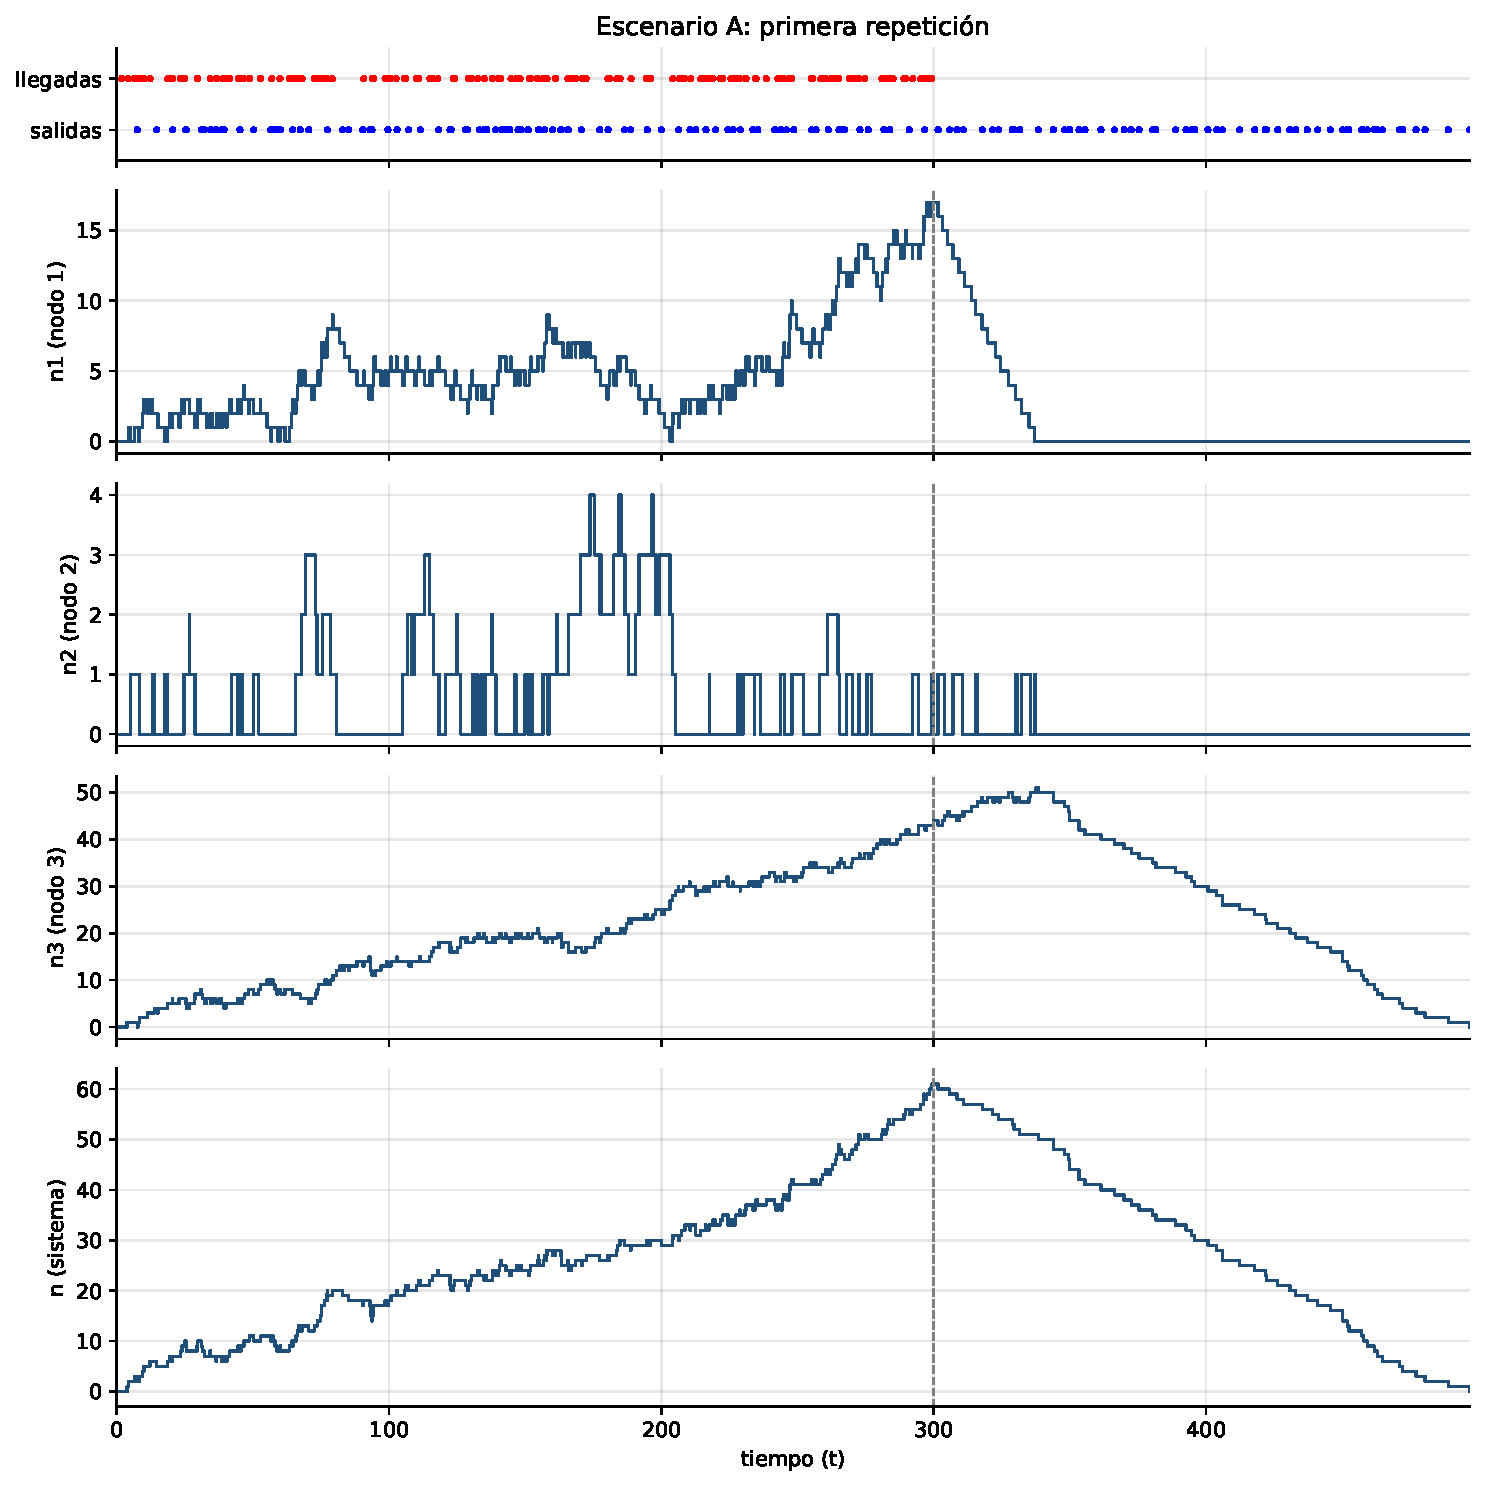
\includegraphics[width=0.84\textwidth]{figuras/52_escA.pdf}
\caption{Escenario A, primera repetición: llegadas y salidas, número de vehículos en cada nodo y en el sistema.}
\label{fig:52A}
\end{figure}

\begin{table}[H]
\centering
\caption{Respuestas a las preguntas con la primera repetición de cada escenario.}
\label{tab:52primera}
\small
\begin{tabular}{@{}>{\raggedright\arraybackslash}p{7cm}rr@{}}
\toprule
Medida & Escenario A & Escenario B \\
\midrule
Tiempo medio en el sistema (\texttt{t\_med\_sistema}) & 87,2638 & 23,2720 \\
Número promedio en el nodo 1 (\texttt{n\_med\_n1}) & 3,7653 & 3,2319 \\
Número promedio en el nodo 2 (\texttt{n\_med\_n2}) & 0,4598 & 0,1787 \\
Número promedio en el nodo 3 (\texttt{n\_med\_n3}) & 23,1522 & 2,9987 \\
Tiempo desde $T$ hasta que sale el último & 196,7626 & 26,7854 \\
Número máximo de clientes en el sistema & 61 & 15 \\
Clientes que pasaron por el nodo 1 ($n_1$) & 156 & 90 \\
Clientes que pasaron por el nodo 2 ($n_2$) & 59 & 36 \\
Clientes que pasaron por el nodo 3 ($n_3$) & 156 & 90 \\
Total de clientes que pasaron por el sistema & 156 & 90 \\
\bottomrule
\end{tabular}
\end{table}

En la figura \ref{fig:52A} se ve dónde está el problema del escenario A. N1 se congestiona por ratos pero se
recupera; N2 pasa el 57\,\% del tiempo vacío; N3, en cambio, crece sin parar hasta $T$. A N3 llegan unos 0,48
vehículos por unidad de tiempo, que es lo que deja salir N1, y aun trabajando rápido ($\mu_{32} = 3$) solo
atiende 0,33. Después de cerrar las llegadas, vaciar la nave principal toma casi 200 unidades de tiempo.

\subsection{Escenario B}

$\lambda = 3$; N1: $N(3{,}0;\ 1{,}0)$; N2: exponencial con $\mu_2 = 1{,}5$; N3: $N(4{,}0;\ 2{,}0)$ si $n_3 < 5$ y
$N(2{,}0;\ 1{,}5)$ si $n_3 \ge 5$.

\begin{figure}[H]
\centering
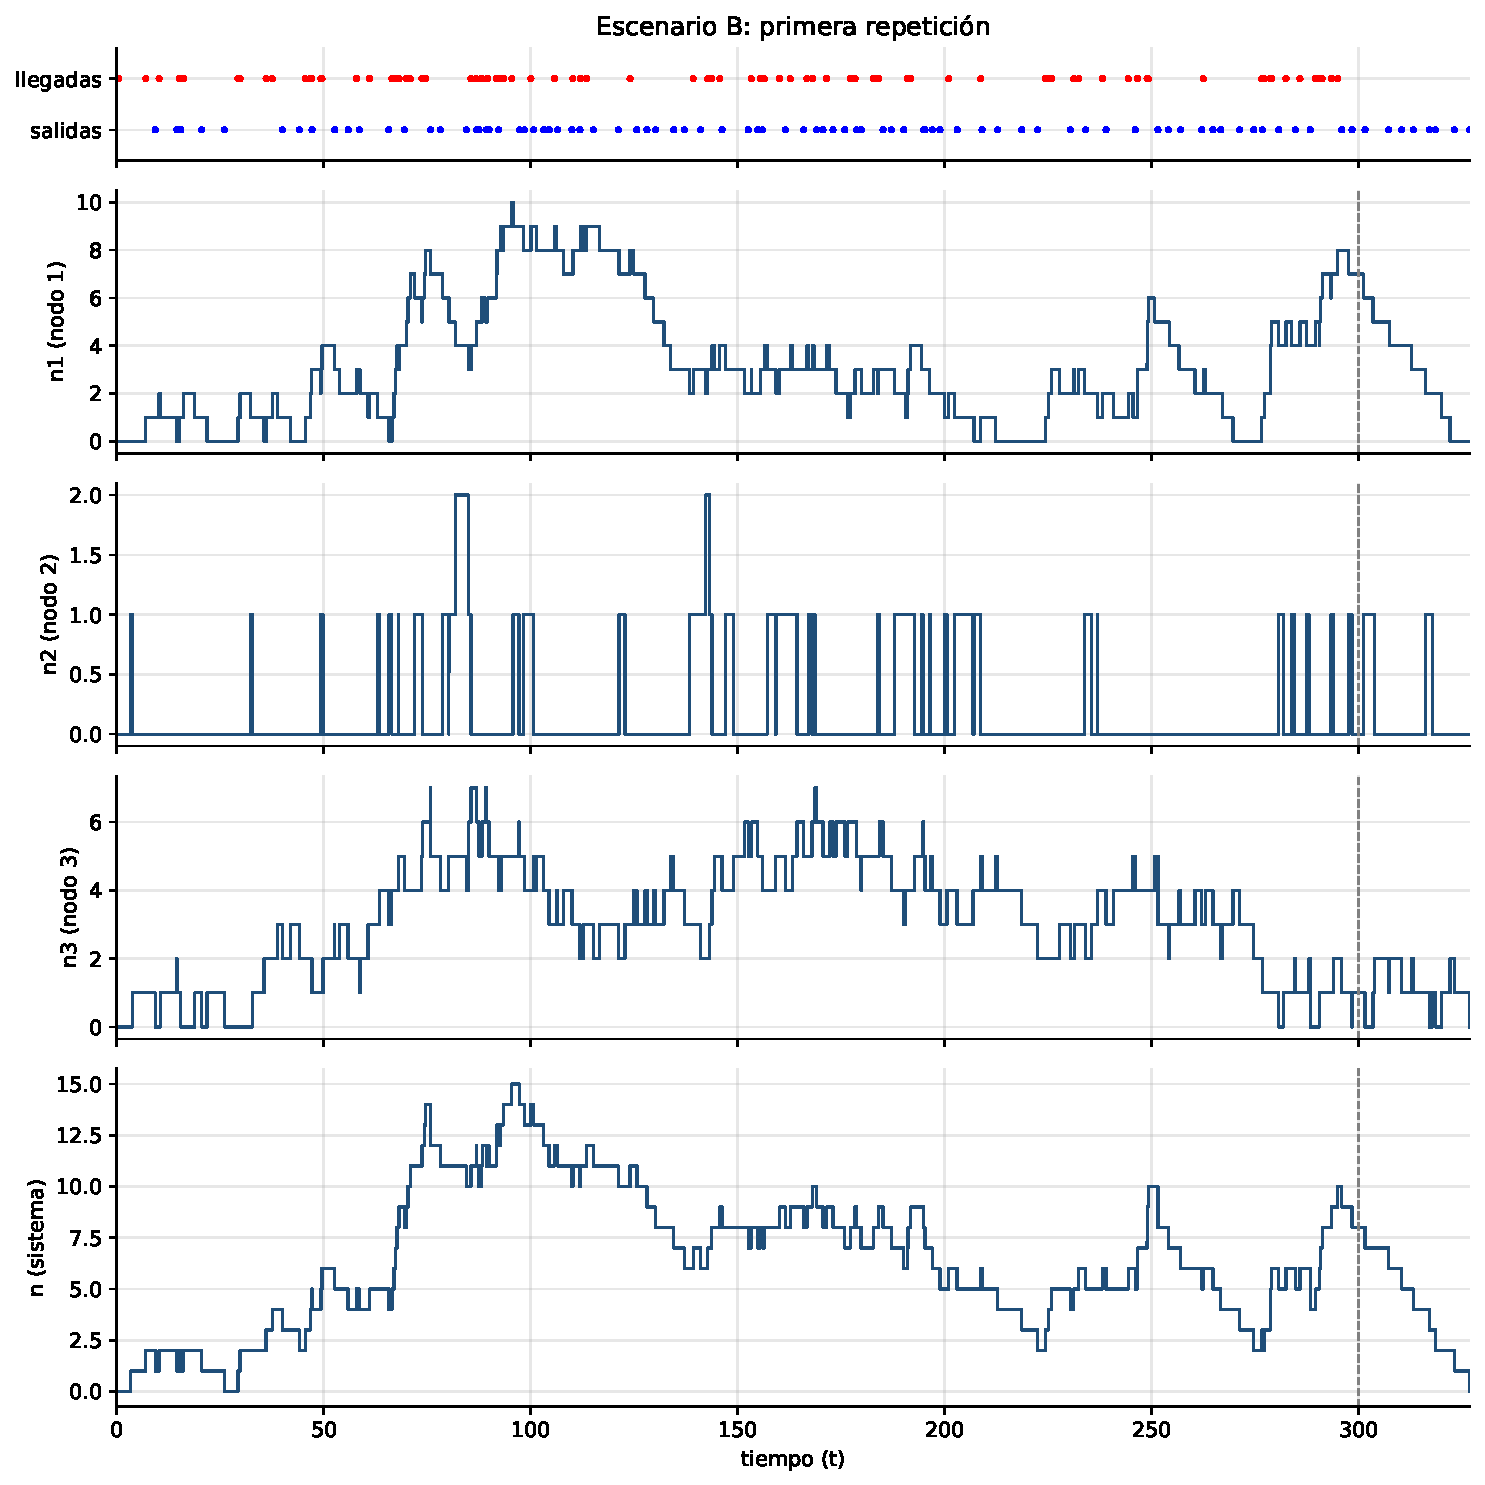
\includegraphics[width=0.84\textwidth]{figuras/52_escB.pdf}
\caption{Escenario B, primera repetición.}
\label{fig:52B}
\end{figure}

El comportamiento es muy distinto. N3 ya no se desborda: pasa cerca del 80\,\% del tiempo con entre 2 y 6
vehículos. El nodo que manda ahora es N1, con $\rho_1 = 3{,}0/3{,}0 = 1$, y en la figura \ref{fig:52B} tiene
las subidas y bajadas largas típicas de una cola en el límite de la estabilidad.

\subsection{Veinte repeticiones por escenario}

Para cada medida se calcularon la media muestral, la desviación estándar muestral y el intervalo de confianza
del 95\,\% con la distribución $t$ de Student:
\[
\bar{x} \pm t_{0{,}975;\,19}\,\frac{s}{\sqrt{20}}, \qquad t_{0{,}975;\,19} = 2{,}093.
\]
La última columna de las tablas \ref{tab:52A} y \ref{tab:52B} es el semiancho del intervalo como porcentaje de
la media, que sirve para comparar la precisión de medidas con escalas distintas.

\begin{table}[H]
\centering
\caption{Escenario A: 20 repeticiones.}
\label{tab:52A}
\small
\begin{tabular}{@{}lrrcr@{}}
\toprule
Medida & Media & Desv. estándar & IC 95\,\% & Semiancho \\
\midrule
\tablain{tablas/tab52_A.tex}
\bottomrule
\end{tabular}
\end{table}

\begin{table}[H]
\centering
\caption{Escenario B: 20 repeticiones.}
\label{tab:52B}
\small
\begin{tabular}{@{}lrrcr@{}}
\toprule
Medida & Media & Desv. estándar & IC 95\,\% & Semiancho \\
\midrule
\tablain{tablas/tab52_B.tex}
\bottomrule
\end{tabular}
\end{table}

\begin{figure}[H]
\centering
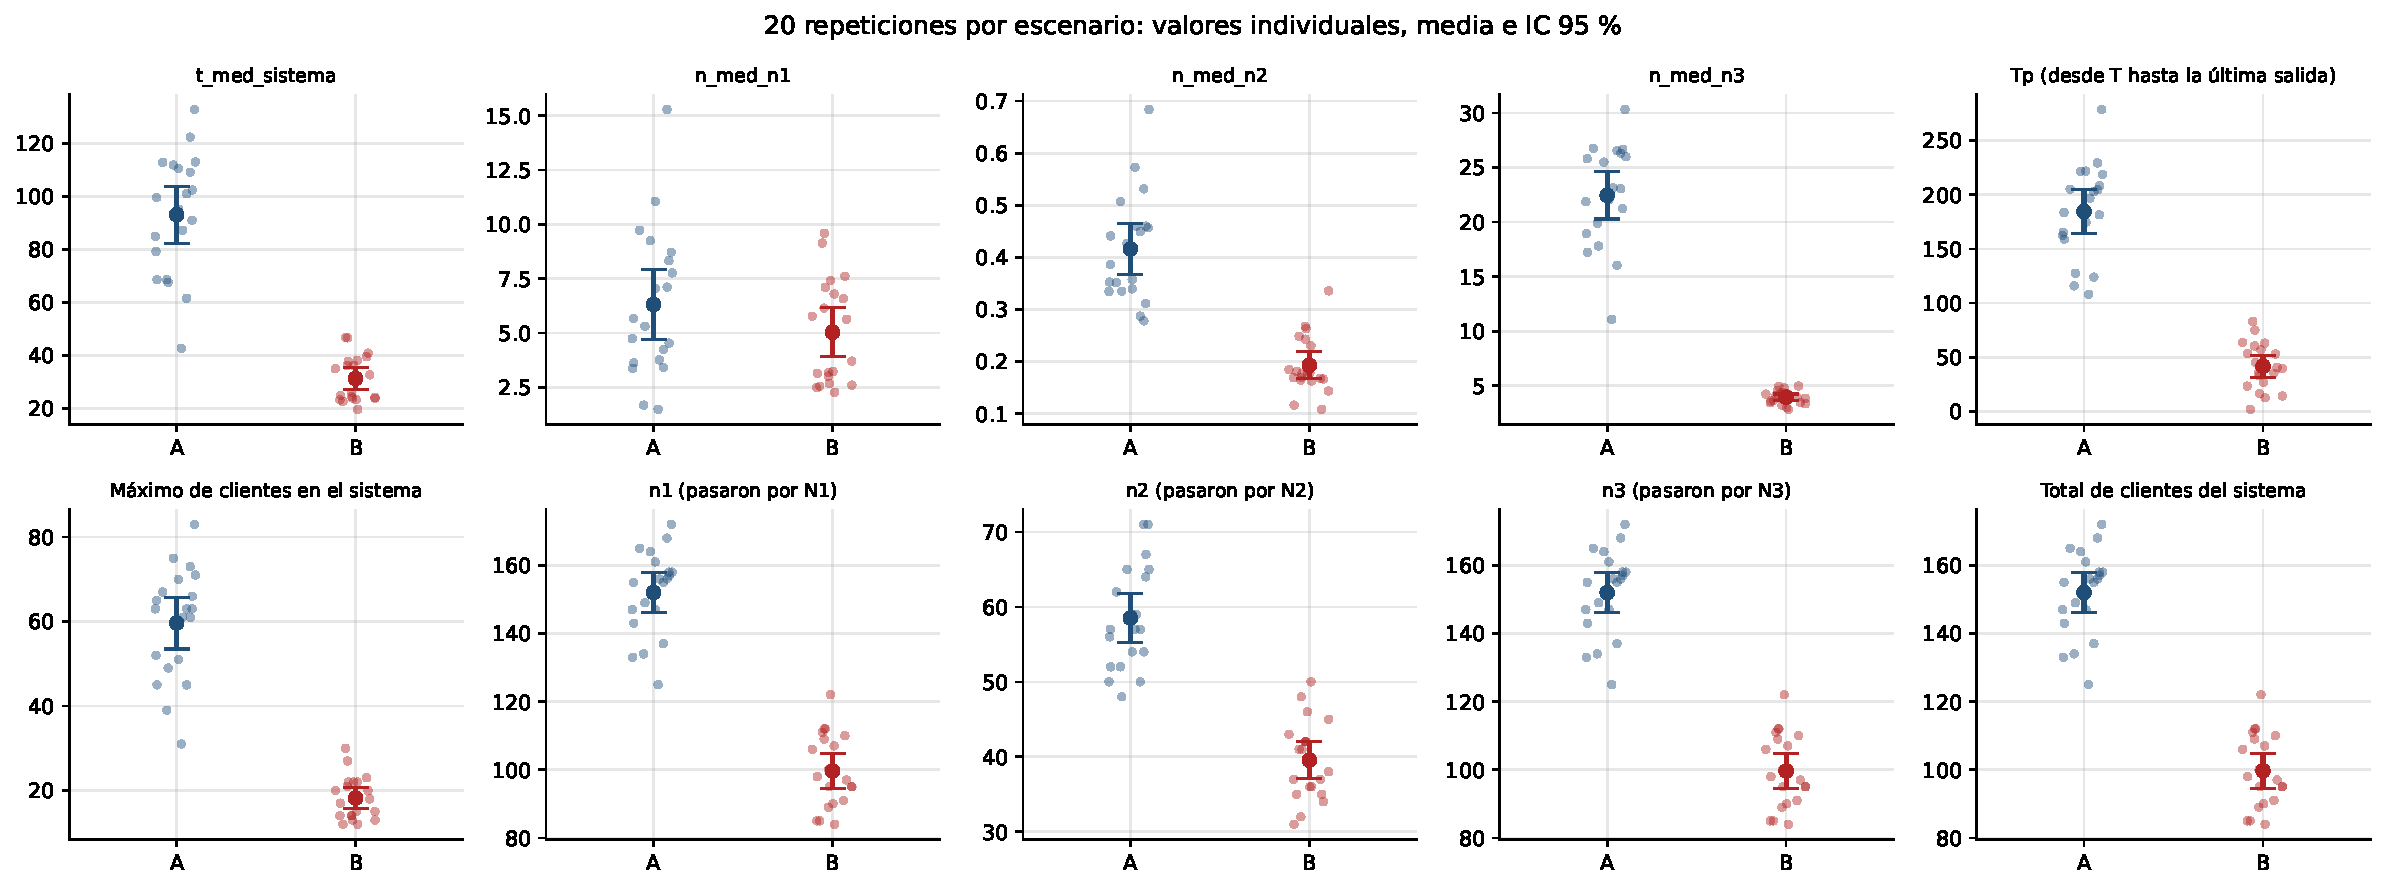
\includegraphics[width=\textwidth]{figuras/52_ic.pdf}
\caption{Valores de las 20 repeticiones (puntos), media e intervalo de confianza del 95\,\% para cada medida y
escenario.}
\label{fig:52ic}
\end{figure}

Como apoyo al análisis se calculó la intensidad de tráfico aproximada de cada nodo, $\rho_j$ = tasa de llegada
al nodo $\times$ tiempo medio de servicio (tabla \ref{tab:52rho}).

\begin{table}[H]
\centering
\caption{Intensidad de tráfico aproximada de cada nodo.}
\label{tab:52rho}
\small
\begin{tabular}{@{}lcc@{}}
\toprule
Nodo & Escenario A & Escenario B \\
\midrule
$\rho_1$ & 1,05 & 1,00 \\
$\rho_2$ & 0,46 & 0,20 \\
$\rho_3$ con $n_3 < 5$ & 1,95 & 1,33 \\
$\rho_3$ con $n_3 \ge 5$ & 1,43 & 0,67 \\
\bottomrule
\end{tabular}
\end{table}

\subsection{¿Qué puede decir de la media y la desviación estándar de la muestra para cada medida?}

\textbf{Los conteos son las medidas más estables y sirven de validación.} Por N1 pasaron $152 \pm 12{,}5$
vehículos en A y $99{,}7 \pm 10{,}9$ en B. Eso es lo que se espera de un proceso de Poisson con
$300/2 = 150$ y $300/3 = 100$ llegadas en promedio, cuya desviación teórica es $\sqrt{150} \approx 12{,}2$ y
$\sqrt{100} = 10$. Por N2 pasó el 38,5\,\% de los vehículos en A y el 39,7\,\% en B, muy cerca del 40\,\% del
modelo. En los dos escenarios $n_3$ y el total del sistema coinciden con $n_1$, porque todos los vehículos
terminan en N3 y la simulación sigue hasta que sale el último.

\textbf{Las medidas de congestión varían mucho más.} El coeficiente de variación está entre 8 y 11\,\% para los
conteos, pero sube a 25\,\% para el tiempo medio en el sistema de A y a 54\,\% para el número medio en N1 de A
($3{,}43/6{,}31$). Estas medidas dependen de cómo se juntan las rachas de llegadas y de servicios largos, no solo
de cuántos vehículos llegan.

\textbf{La mayor variabilidad relativa está siempre en N1}, que en los dos escenarios trabaja con
$\rho_1 \approx 1$. Una cola en ese punto se comporta casi como una caminata aleatoria: puede pasar largos ratos
vacía o acumular muchos vehículos según la suerte de la corrida. En la repetición 5 de A, N1 tuvo en promedio
15,3 vehículos y en la 7 solo 1,5.

\textbf{En N3 se ve el efecto de la regla de los operarios.} En A tiene la media más alta (22,4 vehículos) pero
una variación relativa baja, porque está siempre saturado: ni con el ritmo rápido alcanza
($\rho_3 = 1{,}43$). En B pasa algo interesante. Con menos de 5 vehículos N3 sería inestable ($\rho_3 = 1{,}33$),
así que la cola crece; al llegar a 5 los operarios aceleran ($\rho_3 = 0{,}67$) y la cola baja. N3 termina
rondando el umbral, con media 3,96 y la desviación más pequeña de todas las medidas de congestión (0,63). La
regla funciona como un regulador.

\subsection{¿Qué análisis puede realizar de los intervalos de confianza del 95\,\%?}

La lectura correcta de un intervalo del 95\,\% es que, si se repitiera muchas veces el experimento completo de
20 corridas, cerca del 95\,\% de los intervalos así construidos contendrían el valor esperado verdadero de la
medida. Como los dos escenarios tienen algún nodo inestable, no existe un régimen estable que estimar; lo que se
estima es el comportamiento de un periodo de 300 unidades de tiempo que arranca vacío.

\textbf{La precisión es muy desigual.} El semiancho relativo va de 3,9\,\% para el número de vehículos en A a
25,4\,\% para el número medio en N1 en A. Para el tiempo medio en el sistema de A el intervalo es
$[82{,}36;\ 103{,}85]$, con un semiancho de 10,7, el 11,5\,\% de la media. Bajar ese error al 5\,\% exigiría unas
$n \approx (2{,}093 \cdot 22{,}96 / (0{,}05 \cdot 93{,}10))^2 \approx 107$ corridas, cinco veces más.

\textbf{Casi todas las diferencias entre A y B son claras.} En 9 de las 10 medidas los intervalos no se
traslapan. El tiempo medio en el sistema está entre 82,4 y 103,9 en A y entre 27,3 y 35,3 en B: B es unas tres
veces mejor para el usuario, aunque su ventanilla sea más lenta (3,0 contra 2,1). La mejora viene de que llegan
menos vehículos y de que N3, el cuello de botella de A, en B atiende más rápido cuando se congestiona
($\mu_{32} = 2{,}0$ contra 3,0).

\textbf{La única medida sin diferencia significativa es el número medio en N1}: $[4{,}70;\ 7{,}91]$ en A y
$[3{,}91;\ 6{,}16]$ en B. En los dos escenarios N1 está en $\rho_1 \approx 1$, y con esa variabilidad 20 corridas no
alcanzan para separar los dos casos. Eso no significa que sean iguales, solo que la muestra no permite afirmar
que sean distintos.

\textbf{Sobre el supuesto de normalidad.} El intervalo $t$ supone que la media muestral es aproximadamente
normal. Para los conteos se cumple bien. Para el tiempo después de $T$ o el número medio en N1, con colas largas
hacia arriba (en B el tiempo después de $T$ fue 12,7 en una repetición y 75,2 en otra), la aproximación con 20
corridas es más dudosa, y esos intervalos conviene tomarlos como orientativos.

% =====================================================
\section{Numeral 5.3: inventario probabilístico}
% =====================================================

\subsection{El modelo y sus parámetros}

Se implementó el modelo de la sección 5.6 de \cite{rios08}. Un almacén vende un producto a $r$ por unidad. Los
clientes llegan según un proceso de Poisson de parámetro $\lambda$ y cada uno pide una cantidad aleatoria con
distribución $G$; si no hay suficiente se le vende lo que queda y el resto de la venta se pierde. Cuando el nivel
del inventario $x$ queda por debajo de $p$ y no hay pedido pendiente, se piden $P - x$ unidades, que llegan
$L$ unidades de tiempo después y se pagan al recibirlas. Además se paga un costo de almacenamiento por unidad y
unidad de tiempo. Los sucesos son dos, la llegada de un cliente ($t_C$) y la llegada de un pedido ($t_P$), y el
programa sigue la misma estructura de los numerales anteriores.

\begin{table}[H]
\centering
\caption{Parámetros de la simulación.}
\label{tab:53par}
\small
\begin{tabular}{@{}clc@{}}
\toprule
Símbolo & Significado & Valor \\
\midrule
$P_0$ & inventario inicial & 20 \\
$P$ & nivel máximo de inventario & 100 \\
$p$ & nivel por debajo del cual se hace un pedido & 20 \\
$L$ & tiempo que tarda en llegar un pedido & 5 \\
$h$ & valor a pagar por unidad, $c(y) = h\,y$ & 100 \\
$r$ & precio de venta al público & 150 \\
\midrule
$\lambda$ & tasa de llegada de clientes & 1 \\
$G$ & demanda de cada cliente & uniforme en $\{1, \dots, 5\}$ \\
$a$ & costo de almacenamiento por unidad y unidad de tiempo & 1 \\
$T$ & horizonte de simulación & 100 \\
\bottomrule
\end{tabular}
\end{table}

Los seis primeros valores son los de la guía. Hay que aclarar dos cosas sobre ellos. La guía describe $p$ como
la ``cantidad de producto a pedir si no hay pedidos pendientes'', pero en el modelo del libro $p$ es el
\textbf{nivel de reorden} y la cantidad pedida es $P - x$; así aparece también en la Figura 1 de la guía, tomada
de la Figura 5.9 del libro, donde los pedidos se marcan como $P - x_1$ y $P - x_2$. Se siguió el libro. La otra
es que en el libro $h$ es el costo de almacenamiento y el costo del pedido es una función aparte $c(y)$; como la
guía define $h = 100$ como el valor a pagar por unidad, se usó $c(y) = 100\,y$ y, para el almacenamiento, que la
guía no da, $a = 1$.

La guía deja $\lambda$ sin valor y tampoco fija $G$ ni $T$. Para la simulación principal se tomó $\lambda = 1$,
demanda uniforme entre 1 y 5 unidades (media 3) y $T = 100$, y al final se repitió el experimento con varios
valores de $\lambda$.

\subsection{Correcciones al pseudocódigo del libro}

Al implementar el pseudocódigo aparecieron tres detalles:

\begin{enumerate}[itemsep=2pt]
\item En \textbf{Llegada\_cliente} la condición de venta completa está escrita como \texttt{demanda < x}, pero
el texto dice ``mayor o igual''. Con \texttt{<}, un cliente que pide exactamente lo que queda se contaría como no
satisfecho. Se usó \texttt{<=}.
\item En \textbf{Llegada\_pedido} aparece \texttt{Si var\_aux > 0}, una variable que no está definida; se
entiende que es \texttt{var\_nivel0}.
\item El libro guarda \texttt{var\_nivel0 = t} cada vez que un cliente encuentra el inventario insuficiente,
también cuando ya estaba en cero, con lo que se pierde el tramo anterior. Aquí se guarda solo cuando el inventario
pasa a cero, incluso si llega a cero con una venta completa.
\end{enumerate}

También se agregó el cierre del periodo: si el último suceso ocurre antes de $T$, se acumula el almacenamiento y
el tiempo en cero hasta $T$, y el porcentaje de inventario en cero se calcula sobre $\max(T, t_{final})$.

\subsection{Resultados de la simulación principal}

\begin{figure}[H]
\centering
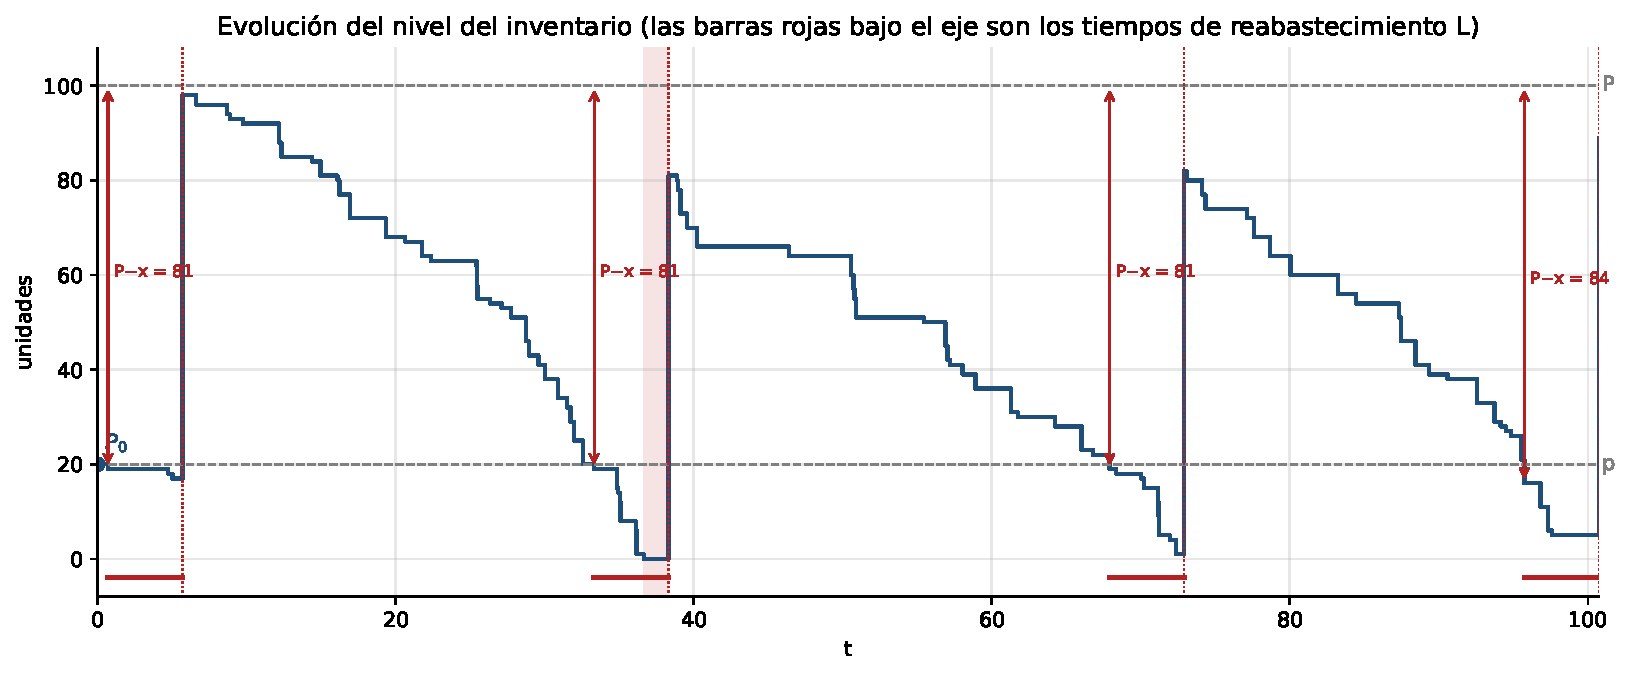
\includegraphics[width=\textwidth]{figuras/53_nivel.pdf}
\caption{Evolución del nivel del inventario, al estilo de la Figura 1 de la guía. Las flechas son los pedidos
de $P - x$ unidades, las barras bajo el eje el tiempo de reabastecimiento $L$ y la franja sombreada el periodo
con el inventario en cero.}
\label{fig:53nivel}
\end{figure}

\begin{figure}[H]
\centering
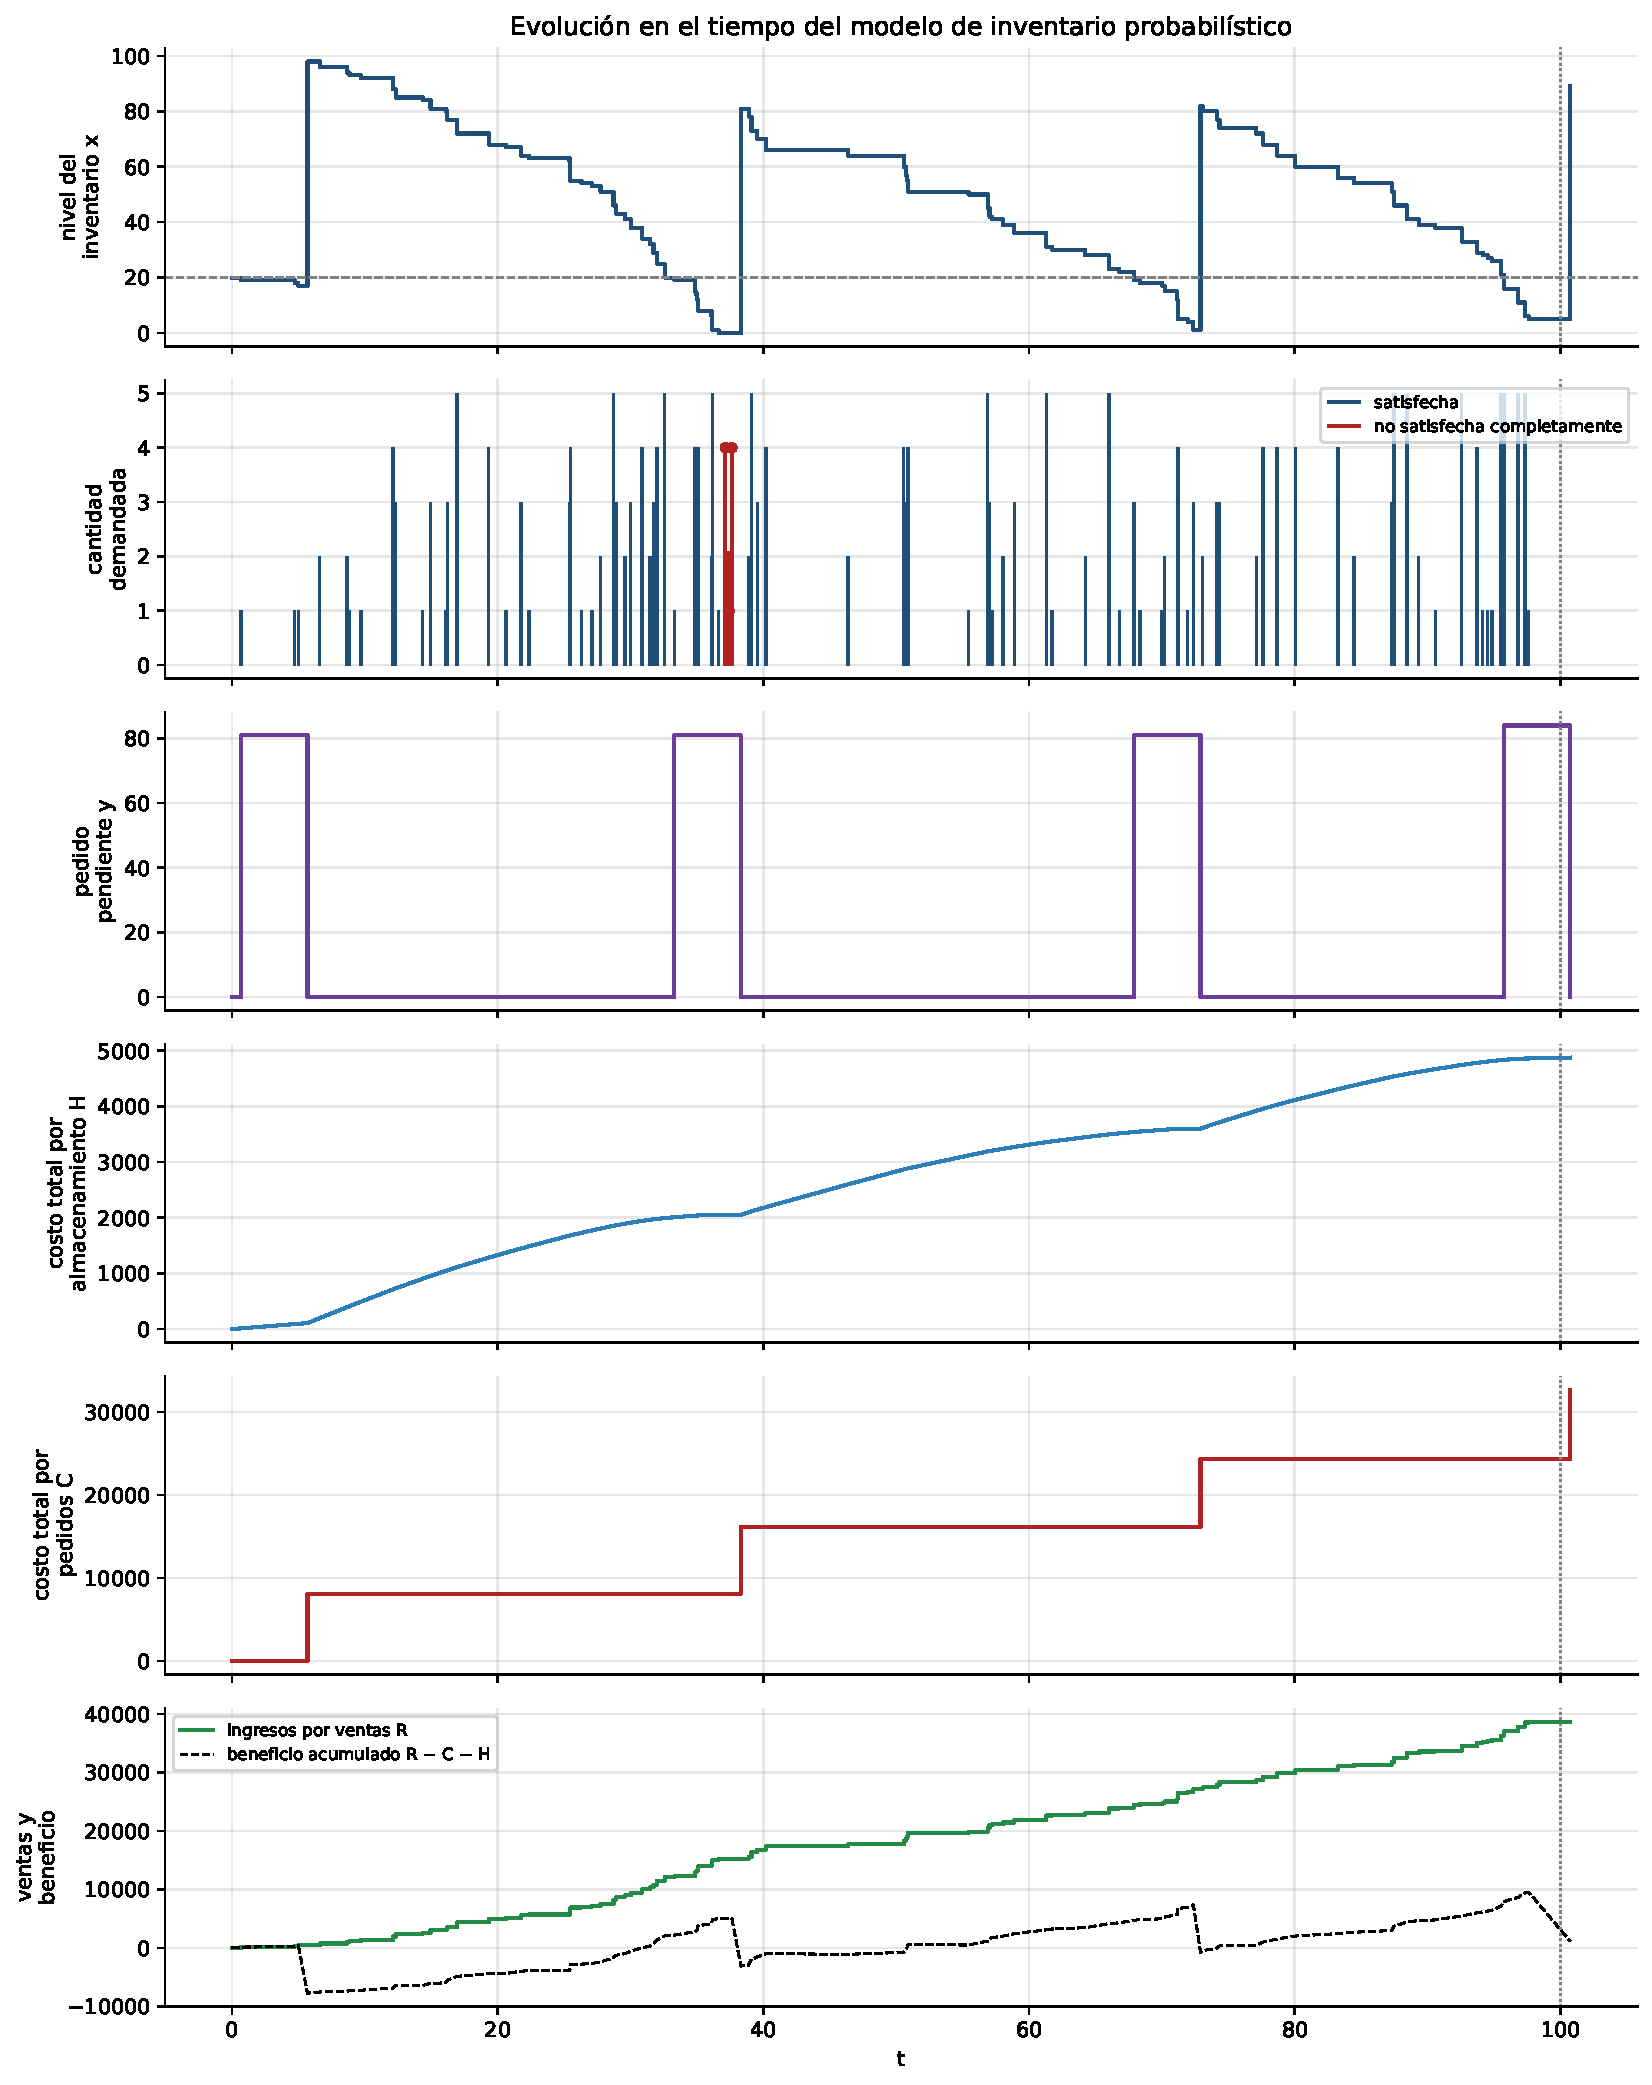
\includegraphics[width=0.93\textwidth]{figuras/53_panel.pdf}
\caption{Evolución en el tiempo de las seis variables que pide la guía: nivel del inventario, cantidad
demandada por cada cliente (en rojo las que no se satisficieron), pedido pendiente, costo total por
almacenamiento, costo total por pedidos, e ingresos por ventas con el beneficio acumulado.}
\label{fig:53panel}
\end{figure}

\begin{table}[H]
\centering
\caption{Medidas de desempeño al final de la simulación principal.}
\label{tab:53med}
\small
\begin{tabular}{@{}lr@{}}
\toprule
Medida & Valor \\
\midrule
\textbf{Beneficio} $R - C - H$ & \textbf{1.121,70} \\
\textbf{Porcentaje de clientes satisfechos} & \textbf{95,96\,\%} (95 de 99) \\
\textbf{Porcentaje de inventario en cero} & \textbf{1,66\,\%} \\
\midrule
Ingresos por ventas $R$ (258 unidades) & 38.700,00 \\
Costo por pedidos $C$ (4 pedidos: 81, 81, 81 y 84 unidades) & 32.700,00 \\
Costo por almacenamiento $H$ & 4.878,30 \\
Inventario final & 89 unidades \\
Beneficio ajustado por inventario final & 8.021,70 \\
\bottomrule
\end{tabular}
\end{table}

El beneficio de 1.121,70 parece bajo, y la razón se ve en el último panel de la figura \ref{fig:53panel}: el
cuarto pedido se hizo en $t = 95{,}74$ y llegó en $t = 100{,}74$, cuando el periodo ya había cerrado. Se pagaron
8.400 por unidades que no se alcanzaron a vender, y la simulación terminó con 89 unidades en bodega. Para
separar ese efecto de borde se calculó un \emph{beneficio ajustado}, $R - C - H + h(x_{final} - P_0)$, que valora a
costo la diferencia entre el inventario final y el inicial; en esta corrida es 8.021,70.

El único desabastecimiento ocurrió entre $t = 37{,}13$ y $t = 38{,}31$. El segundo pedido se hizo en
$t = 33{,}31$ con 19 unidades en bodega, y en las cinco unidades de tiempo que tardó en llegar la demanda se las
llevó todas. Los cuatro clientes no satisfechos llegaron en ese hueco. Los otros tres pedidos llegaron cuando aún
quedaban 17, 1 y 5 unidades.

\subsection{Réplicas y efecto de la tasa de llegada}

El libro cierra la sección indicando que hay que replicar la simulación para estimar las medidas. Se hicieron 30
réplicas con $\lambda = 1$ (tabla \ref{tab:53rep}) y, como la guía deja $\lambda$ libre, otras 30 para cada
$\lambda \in \{0{,}5;\ 1;\ 1{,}5;\ 2;\ 3\}$ (tabla \ref{tab:53lam} y figura \ref{fig:53lam}).

\begin{table}[H]
\centering
\caption{30 réplicas con $\lambda = 1$ y $T = 100$.}
\label{tab:53rep}
\small
\begin{tabular}{@{}lrrc@{}}
\toprule
Medida & Media & Desv. estándar & IC 95\,\% \\
\midrule
\tablain{tablas/tab53_replicas.tex}
\bottomrule
\end{tabular}
\end{table}

\begin{table}[H]
\centering
\caption{Promedio de 30 réplicas para distintos valores de $\lambda$.}
\label{tab:53lam}
\small
\begin{tabular}{@{}crrrrr@{}}
\toprule
$\lambda$ & Beneficio & Benef. ajustado & Satisfechos (\%) & Inventario en cero (\%) & Pedidos \\
\midrule
\tablain{tablas/tab53_lambda.tex}
\bottomrule
\end{tabular}
\end{table}

\begin{figure}[H]
\centering
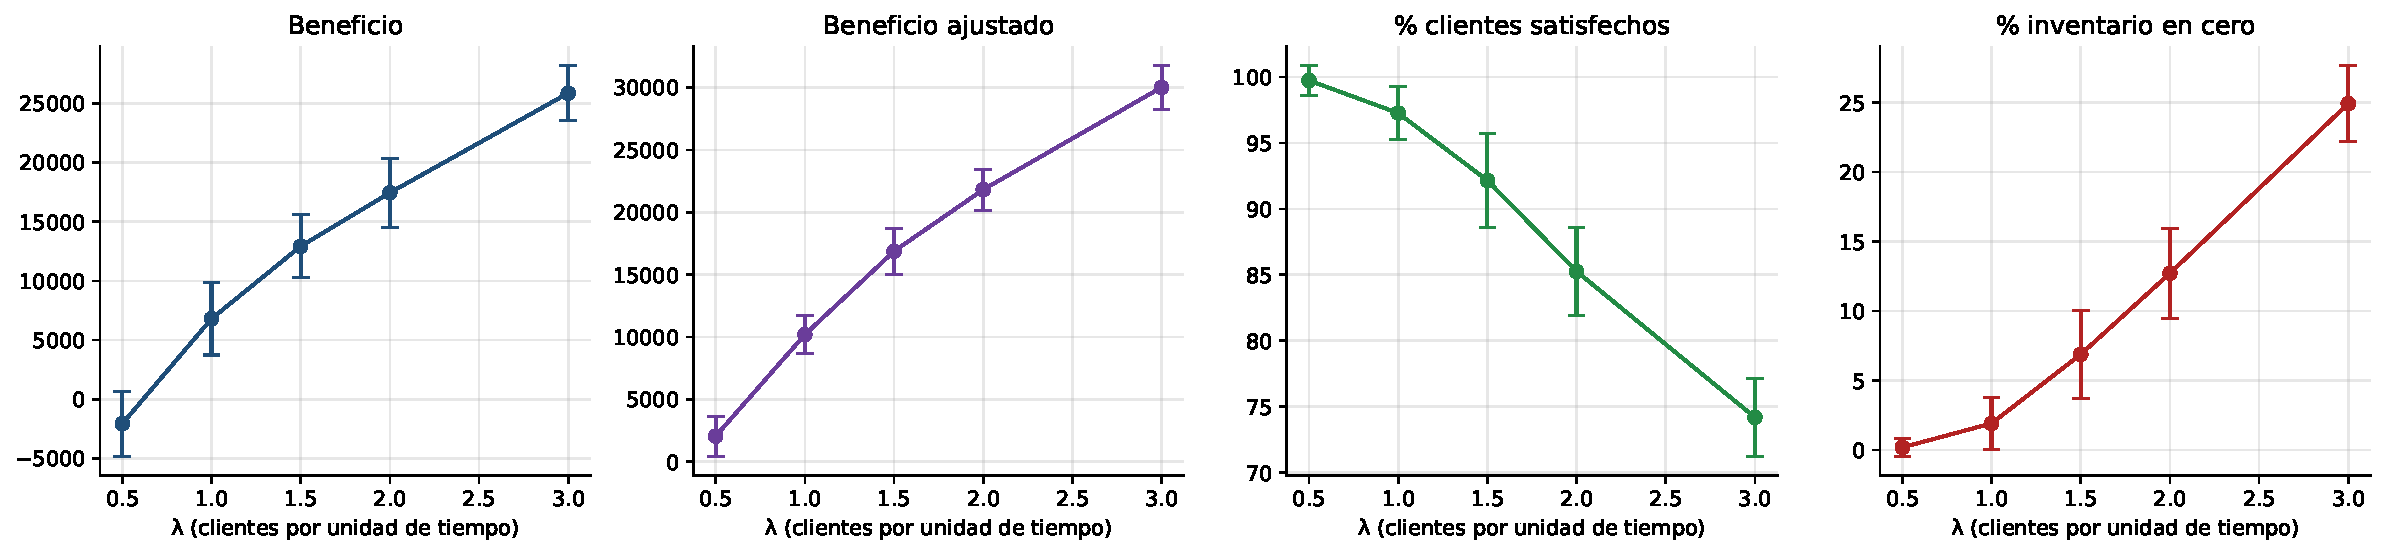
\includegraphics[width=\textwidth]{figuras/53_lambda.pdf}
\caption{Medidas de desempeño en función de $\lambda$ (media $\pm$ una desviación estándar, 30 réplicas).}
\label{fig:53lam}
\end{figure}

\subsection{Análisis}

\textbf{Una sola corrida no basta para evaluar el beneficio.} En las 30 réplicas con $\lambda = 1$ el beneficio
fue $6.799{,}61 \pm 3.063{,}02$, con un intervalo del 95\,\% de $[5.655{,}86;\ 7.943{,}36]$, y la corrida
principal quedó muy por debajo por el pedido de fin de periodo. Buena parte de la variabilidad viene de ese
efecto de borde: el beneficio ajustado tiene la mitad de desviación (1.549,03). Esto sugiere que la política
debería considerar el horizonte, por ejemplo no hacer pedidos si faltan menos de $L$ unidades de tiempo para
cerrar.

\textbf{Con $\lambda = 1$ la política $(p = 20, P = 100)$ da un buen servicio:} 97,27\,\% de clientes
satisfechos (IC: 96,51 a 98,02) y el inventario en cero solo el 1,92\,\% del tiempo. Durante las $L = 5$
unidades de tiempo de espera de un pedido se demandan en promedio $\lambda L\,E[D] = 1 \cdot 5 \cdot 3 = 15$
unidades, menos que las 20 con que se dispara el pedido. Solo cuando la demanda de ese plazo sale alta hay
faltantes, como pasó en la corrida principal.

\textbf{El efecto de $\lambda$ confirma ese razonamiento.} La demanda esperada durante el plazo de entrega es
$15\lambda$, que supera el punto de reorden cuando $\lambda > 4/3$. La tabla \ref{tab:53lam} muestra el quiebre
justo ahí: el tiempo con inventario en cero pasa de 1,9\,\% con $\lambda = 1$ a 6,9\,\% con $\lambda = 1{,}5$,
12,7\,\% con $\lambda = 2$ y 24,9\,\% con $\lambda = 3$, y los clientes satisfechos bajan de 97,3\,\% a 74,2\,\%.
El beneficio sí crece con $\lambda$ porque se venden más unidades con un margen de 50 cada una, pero con
$\lambda = 3$ uno de cada cuatro clientes se va sin su pedido completo.

\textbf{Con poca demanda el negocio pierde.} Con $\lambda = 0{,}5$ el beneficio medio fue negativo ($-2.072$).
Se vendieron en promedio 152 unidades por 22.780, pero los pedidos costaron 19.307 y el almacenamiento 5.546,
porque cada pedido de unas 80 unidades tarda unas 53 unidades de tiempo en venderse. Además se terminó con 61
unidades sin vender en promedio. Para esa demanda convendría un $P$ más bajo.

En resumen, con los valores de la guía $p = 20$ solo es adecuado si llegan a lo sumo 1,3 clientes por unidad de
tiempo. Para demandas mayores habría que subir el punto de reorden al menos a $15\lambda$ más un margen de
seguridad, o conseguir un proveedor con menor $L$. El modelo permite probar esas políticas cambiando dos
parámetros, que es justamente el uso que le da el libro: ayudar a redefinir la política de gestión del
inventario.

% =====================================================
\section{Numeral 5.4: simulación de eventos discretos en SimPy}
% =====================================================

Todo este numeral está en el cuaderno \texttt{Lab4\_5.4\_SimPy\_\codigoEstudiante.ipynb}. Aquí se resume cada
parte con los fragmentos de código y las salidas más importantes.

\subsection{Instalación}

SimPy se instala con \texttt{pip install simpy} tanto en Colab como en un equipo local. Se trabajó con SimPy
4.1.2 sobre Python 3.13.

\subsection{Tutorial de Stefan Scherfke}

Se siguió la presentación \emph{Discrete-event simulation with SimPy} (EuroPython 2014) paso a paso, junto con el
cuaderno \emph{Discrete-event simulation with SimPy.ipynb} del curso, que traduce los mismos ejemplos:

\begin{enumerate}[itemsep=2pt]
\item \textbf{Funciones generadoras.} \texttt{yield} entrega un valor y congela la función; \texttt{send()} le
devuelve un valor. Con \texttt{generator(1)} se obtuvo 2 con \texttt{next} y \texttt{StopIteration} con valor 4
al enviar 3. Es el mecanismo con que SimPy suspende y reanuda procesos.
\item \textbf{Primer modelo: dos relojes.} Dos procesos con \texttt{env.timeout(0.5)} y \texttt{env.timeout(1)} se
intercalan según el tiempo simulado: \texttt{rápido 0, lento 0, rápido 0.5, lento 1, rápido 1.0, rápido 1.5}.
\item \textbf{\texttt{Environment} y \texttt{RealtimeEnvironment}.} Con el mismo modelo, 10 unidades simuladas
tomaron 0,000\,s en el primero y 1,000\,s en el segundo con \texttt{factor=0.1}.
\item \textbf{Los timeouts dejan pasar el tiempo; los procesos también son eventos.} Un orador espera su turno
y habla 30 minutos; un moderador espera a cada orador con \texttt{yield env.process(...)} y recibe su valor de
retorno.
\item \textbf{Interrupciones.} El moderador corta a cada orador a los 30 minutos con \texttt{interrupt()}.
\item \textbf{Eventos de condición.} \texttt{speaker\_proc | env.timeout(30)} espera lo que ocurra primero.
\item \textbf{Recursos compartidos:} ejemplos cortos con \texttt{Resource}, \texttt{Container} y \texttt{Store}.
\item \textbf{Asistente a la conferencia}, con y sin \emph{buffet} limitado.
\end{enumerate}

En los pasos 5 y 6 aparecieron dos detalles que valen la pena. Con la versión de las diapositivas que
interrumpe siempre a los 30 minutos, el segundo orador terminó solo en $t = 57$ y el moderador intentó
interrumpirlo en $t = 60$; SimPy lanza un \texttt{RuntimeError}, porque no se puede interrumpir un proceso
terminado. El evento de condición lo resuelve casi siempre, pero no cuando hay \textbf{empate}: con la semilla
usada, el quinto orador habló exactamente 30 minutos. En $t = 145$ ocurren dos eventos a la vez; la condición se
dispara con el \emph{timeout}, que SimPy procesa primero, así que \texttt{results} no incluye al orador, pero
antes de que el moderador reanude la charla ya terminó, y el error vuelve a aparecer. La versión robusta pregunta
además si el proceso sigue vivo:

\begin{lstlisting}
results = yield speaker_proc | env.timeout(30)
if speaker_proc not in results and speaker_proc.is_alive:
    speaker_proc.interrupt('No queda tiempo')
\end{lstlisting}

En el ejemplo del \emph{buffet} con un solo puesto y 3 minutos por persona, la ventana de $15 - 3 = 12$ minutos
solo alcanza para 4 de los 5 asistentes. Los cuatro primeros comen en $t = 93, 96, 99$ y $102$, y el quinto se
queda sin comer en las dos sesiones, porque todos terminan las charlas a la vez y SimPy atiende las peticiones
en el orden en que se hicieron. En las diapositivas, además, la línea
\texttt{time\_left = LEN\_BREAK - (env.now - start)} usa una constante que no existe; debe ser
\texttt{BREAK\_LENGTH}, como ya está en el cuaderno del curso.

\subsection{Tutorial \emph{SimPy in 10 minutes}}

\begin{enumerate}[itemsep=2pt]
\item \textbf{Conceptos básicos.} Un proceso \texttt{car} que alterna 5 unidades estacionado y 2 conduciendo:
empieza a conducir en 5, estaciona en 7, conduce en 12 y estaciona en 14.
\item \textbf{Interacción entre procesos.} El carro eléctrico espera al proceso \texttt{charge}, y un conductor
lo interrumpe en $t = 3$; el carro atrapa la excepción \texttt{simpy.Interrupt} y sale a conducir en $t = 3$ en
vez de en 5.
\item \textbf{Recursos compartidos.} Una estación de carga con dos puestos
(\texttt{simpy.Resource(env, capacity=2)}) y cuatro carros que llegan en $t = 0, 2, 4, 6$ con cargas de 5.
\end{enumerate}

\begin{lstlisting}
def car(env, name, bcs, driving_time, charge_duration):
    yield env.timeout(driving_time)
    with bcs.request() as req:        # pedir un puesto de carga
        yield req                      # esperar hasta obtenerlo
        yield env.timeout(charge_duration)
\end{lstlisting}

El carro 2 llega en $t = 4$ con los dos puestos ocupados y empieza en $t = 5$, cuando sale el carro 0; el carro 3
llega en 6 y empieza en 7. Cada uno espera exactamente una unidad de tiempo, lo mismo que da la cuenta a mano.

\subsection{Ejemplos de SimPy}

Los siete ejemplos se implementaron con el código de la documentación oficial y se ejecutaron sin cambios, para
poder comparar la salida con la publicada (coincide, porque todos fijan \texttt{RANDOM\_SEED = 42}). La tabla
\ref{tab:simpy} resume qué modela cada uno y qué se obtuvo.

\begin{longtable}{@{}>{\raggedright\arraybackslash}p{2.6cm}>{\raggedright\arraybackslash}p{5.6cm}>{\raggedright\arraybackslash}p{7.2cm}@{}}
\caption{Ejemplos de SimPy implementados.}\label{tab:simpy}\\
\toprule
Ejemplo & Qué modela y qué usa & Resultado \\
\midrule
\endfirsthead
\toprule
Ejemplo & Qué modela y qué usa & Resultado \\
\midrule
\endhead
Bank Renege & Mostrador único; clientes con paciencia entre 1 y 3 que abandonan. \texttt{Resource} y evento de
condición \texttt{req | timeout(patience)}. & De 5 clientes, 4 fueron atendidos sin esperar y el cliente 2
abandonó en $t = 13{,}90$ tras esperar 1,17 mientras el cliente 1 estaba en el mostrador. \\
\addlinespace
Carwash & Lavadero con 2 máquinas, lavado de 5 minutos, 4 carros iniciales y uno cada 5 a 9 minutos.
\texttt{Resource} y espera de otro proceso. & Los carros 2 y 3 esperan hasta $t = 5$ y el 4 hasta $t = 10$;
después la cola desaparece, porque la capacidad (0,4 carros/min) supera las llegadas (0,14 carros/min). \\
\addlinespace
Machine Shop & 10 máquinas que se dañan cada 300 min en promedio y un técnico que las repara en 30 min.
\texttt{interrupt()} y \texttt{PreemptiveResource} con prioridades. & En 4 semanas cada máquina hizo en promedio
3277,5 piezas, el 81\,\% de las 4032 que haría sin daños. El técnico recibe $10 \cdot 30/300 = 1$ hora de
reparación por hora: está saturado. \\
\addlinespace
Movie Renege & Taquilla con 3 películas de 50 boletas; al agotarse una, todos los que esperaban por ella se van.
\texttt{Resource}, evento compartido y condición. & Se agotaron a los 28, 38 y 43 minutos; se fueron de la fila
5, 16 y 5 personas cuando se agotaron. \\
\addlinespace
Gas Station Refueling & 2 surtidores con tanque común de 200 L y carrotanque que tarda 300 s.
\texttt{Resource}, \texttt{Container} y proceso de control. & El tanque bajó a 12 L en $t = 459$ y se llamó al
carrotanque en $t = 460$; llegó en $t = 760$ con 188 L. Los carros 5 y 6 quedaron esperando combustible; el 5
esperó 55 s. \\
\addlinespace
Process Communication & Mensajes uno a uno y uno a muchos. \texttt{Store} como tubería y búfer. & Los mensajes
que el consumidor no alcanza a leer esperan en el \texttt{Store} y se marcan como \emph{LATE} (por ejemplo, el de
$t = 65$ leído en 66). En el caso uno a muchos cada consumidor tiene su propio \texttt{Store}. \\
\addlinespace
Event Latency & Cable con retardo de 10 unidades entre emisor y receptor. \texttt{Store} y un proceso por
mensaje. & Cada mensaje enviado cada 5 unidades llega exactamente 10 después; el retardo vive en la clase
\texttt{Cable}, no en los procesos. \\
\bottomrule
\end{longtable}

La diferencia con los numerales 5.1 a 5.3 está en el enfoque. Allá se programaba a mano la lista de sucesos, el
reloj y la elección del suceso más próximo, lo que se conoce como \textbf{programación de eventos}. En SimPy se
describe lo que hace cada entidad (llegar, pedir un recurso, esperar, salir) y la librería se encarga del reloj y
de la cola de eventos, lo que se conoce como \textbf{interacción de procesos}. Por eso un modelo con
interrupciones y prioridades como el taller de máquinas cabe en unas 100 líneas.

% =====================================================
\section{Numeral 5.5: simulación de eventos discretos en AnyLogic}
% =====================================================

Se instaló AnyLogic 8.9 PLE y se desarrollaron paso a paso los cinco tutoriales de la guía, que vienen en la
ayuda del programa (\emph{Help} $\rightarrow$ \emph{Tutorials}). Los modelos terminados se entregan en la carpeta
\texttt{Modelos\_AnyLogic}.

\subsection{Bank office model (sistema de colas)}

Modela una oficina bancaria con un cajero automático y cuatro cajeros humanos. Se construyó en cuatro fases:

\begin{enumerate}[itemsep=2pt]
\item \textbf{Modelo simple.} Diagrama \texttt{Source} $\rightarrow$ \texttt{Queue} $\rightarrow$
\texttt{Delay} (\texttt{ATM}) $\rightarrow$ \texttt{Sink}, con unidades de tiempo en minutos. Llegan 0,3
clientes por minuto, la cola admite 15 y el cajero automático tarda \texttt{triangular(0.8, 1.5, 3.5)} minutos.
\item \textbf{Animación.} El cajero automático se dibujó como un \emph{Point Node} que cambia de color con
\texttt{ATM.size() > 0 ? red : green} y la cola como un \emph{Path}. Se añadió una ventana 3D, un tipo de agente
\texttt{Customer} con figura de persona y el objeto 3D del cajero automático.
\item \textbf{Cajeros.} Un \texttt{SelectOutput} envía la mitad de los clientes al cajero automático y la otra
mitad a un bloque \texttt{Service} (cola de 20, servicio \texttt{triangular(2.5, 6, 11)} minutos) que toma una
unidad de un \texttt{ResourcePool} de 4 cajeros. La animación usa nodos rectangulares con atractores.
\item \textbf{Estadísticas.} Dos gráficas de barras con \path{ATM.statsUtilization.mean()} y
\path{queue.statsSize.mean()}, y un histograma del tiempo en el sistema medido entre un
\texttt{TimeMeasureStart} y un \texttt{TimeMeasureEnd}.
\end{enumerate}

Hay un detalle de los parámetros. El tutorial dice que el tiempo del cajero automático tiene ``media'' 1,5, pero
según la ayuda de AnyLogic \texttt{triangular(0.8, 1.5, 3.5)} usa 1,5 como moda, así que la media real es
$(0{,}8 + 1{,}5 + 3{,}5)/3 = 1{,}93$ minutos. Con eso se pueden anticipar las utilizaciones: en la fase 1 el cajero
automático recibe 0,3 clientes por minuto y su utilización debería rondar $0{,}3 \cdot 1{,}93 = 0{,}58$. En la
fase 3 recibe la mitad, así que debería bajar a cerca de 0,29, y cada cajero humano tendría
$0{,}15 \cdot 6{,}5 / 4 \approx 0{,}24$.

\captura{al_bank_f1.png}{Bank office, fase 1: diagrama de flujo en ejecución.}
\captura{al_bank_f2.png}{Bank office, fase 2: animación 3D del cajero automático y la cola.}
\captura{al_bank_f3.png}{Bank office, fase 3: modelo con cajeros automáticos y humanos.}
\captura{al_bank_f4.png}{Bank office, fase 4: utilización del cajero automático, longitud media de la cola e
histograma del tiempo en el sistema.}

En las capturas se ve que cada fase hace lo que debe. En la fase 3 el \texttt{selectOutput} repartió 59 clientes
en 30 hacia el cajero automático y 29 hacia los cajeros, que es la mitad esperada con probabilidad 0,5. En la
fase 4, con esos mismos 59 clientes (unas tres horas simuladas), las gráficas dieron una utilización del cajero
automático de 0,24, una longitud media de la cola de 0,04 y un tiempo medio en el sistema de 4,38 minutos.

Esas cifras se pueden contrastar con la teoría. Para la cola del cajero automático, que recibe
$\lambda = 0{,}15$ clientes por minuto, la fórmula de Pollaczek--Khinchine de la cola M/G/1 da
\[
L_q = \frac{\lambda^2 E[S^2]}{2(1-\rho)} = \frac{0{,}15^2 \cdot 4{,}064}{2(1 - 0{,}29)} \approx 0{,}064,
\]
donde $E[S^2] = \operatorname{Var}(S) + E[S]^2 = 0{,}327 + 1{,}933^2$ para la triangular $(0{,}8;\ 1{,}5;\ 3{,}5)$. El
tiempo en el sistema esperado es el promedio de las dos ramas: $1{,}93 + L_q/\lambda \approx 2{,}36$ minutos por el
cajero automático y unos 6,5 por los cajeros, donde casi no se espera porque cada uno trabaja al 24\,\%. Eso da
$0{,}5 \cdot 2{,}36 + 0{,}5 \cdot 6{,}5 \approx 4{,}43$ minutos, muy cerca de los 4,38 simulados. La utilización
(0,24 contra 0,29) y la cola (0,04 contra 0,064) quedaron algo por debajo, lo que es normal con una corrida de
solo 59 clientes. El histograma muestra las dos ramas: un pico alrededor de 2 a 3 minutos, de los clientes del
cajero automático, y una masa más ancha entre 4 y 10 minutos, de los que pasan por los cajeros.

\subsection{Subway entrance (peatones)}

Modela el vestíbulo de entrada de una estación de metro con la \emph{Pedestrian Library}, en cuatro fases:

\begin{enumerate}[itemsep=2pt]
\item \textbf{Flujo simple.} Sobre la imagen del plano se dibujaron las paredes, una línea de entrada y una de
destino. El diagrama \texttt{PedSource} $\rightarrow$ \texttt{PedGoTo} $\rightarrow$ \texttt{PedSink} genera
4000 pasajeros por hora que cruzan el vestíbulo.
\item \textbf{Torniquetes.} Se dibujó un \emph{Service With Lines} lineal con los torniquetes y se agregó un bloque
\texttt{PedService} (\texttt{atFareGates}) con tiempo uniforme entre 2 y 3 segundos.
\item \textbf{Mapa de densidad.} Un \emph{Density map} muestra con colores dónde se aglomeran los pasajeros.
\item \textbf{Máquinas expendedoras.} Un \texttt{PedSelectOutput} manda el 10\,\% de los pasajeros, los que no
tienen tiquete, a un \texttt{PedService} con máquinas expendedoras de tiempo \texttt{triangular(7, 12, 40)}
segundos antes de los torniquetes.
\end{enumerate}

\captura{al_ped_f1.png}{Subway entrance, fase 1: flujo simple de peatones.}
\captura{al_ped_f2.png}{Subway entrance, fase 2: filas en los torniquetes.}
\captura{al_ped_f3.png}{Subway entrance, fase 3: mapa de densidad de peatones.}
\captura{al_ped_f4.png}{Subway entrance, fase 4: modelo completo con máquinas expendedoras.}

En la fase 1, sin ningún obstáculo, los pasajeros cruzan el vestíbulo de la línea de entrada a la de destino
sin detenerse: en la captura se habían generado 813 y en ese instante había 90 caminando. Al poner los
torniquetes en la fase 2 aparecen las filas. Dentro del bloque \texttt{atFareGates} llegó a haber 113 personas
entre las que hacían fila y las que pasaban, y en la fase 3 se mantuvo alrededor de 108 después de más de 2000
pasajeros, así que la fila no se disolvía. El mapa de densidad muestra dónde está el problema: la franja roja,
con más de un pasajero por metro cuadrado, queda justo antes de los torniquetes, y la parte media del vestíbulo
también se carga porque la gente se va represando desde allí. Es la misma conclusión del tutorial: con 4000
pasajeros por hora, el número de torniquetes del modelo apenas alcanza.

En la fase 4 el \texttt{PedSelectOutput} desvió a las máquinas 359 de 3762 pasajeros, el 9,5\,\%, muy cerca del 10\,\%
configurado. Las máquinas tenían 12 personas en ese momento. Como su tiempo de servicio, triangular de 7 a 40
segundos con moda 12, tiene una media de 19,7 segundos, mucho mayor que los 2 a 3 segundos de un torniquete, una
fracción pequeña de pasajeros basta para formar una fila propia. En el mapa de esta fase aparece una zona ocupada
nueva, en la parte superior del vestíbulo donde están las máquinas, y el total de pasajeros que llega a los
torniquetes no cambia, porque los que compran tiquete igual terminan pasando por ellos.

\subsection{Intersection (tráfico vehicular)}

Modela una intersección real (Tapiolavagen y Menninkaisentie) con la \emph{Road Traffic Library}, con unidades
de tiempo en segundos:

\begin{enumerate}[itemsep=2pt]
\item \textbf{Carretera.} Sobre la imagen del plano se dibujó la vía y un diagrama \texttt{CarSource}
$\rightarrow$ \texttt{CarMoveTo} $\rightarrow$ \texttt{CarDispose}.
\item \textbf{Animación 3D} con un tipo de agente \texttt{Car} con figura 3D.
\item \textbf{Intersección.} Al conectar la segunda vía se crea la intersección automáticamente. Los bloques
\texttt{SelectOutput} dejan seguir al 70\,\% de los carros por la vía principal y desvían al 30\,\% hacia la vía
secundaria.
\item \textbf{Parqueadero.} Un \emph{Parking lot} al lado de la vía, al que va el 10\,\% de los carros, con un
\texttt{Delay} de capacidad 5 que representa el tiempo estacionado.
\item \textbf{Buses.} Un segundo \texttt{CarSource} genera 20 buses por hora de 10 metros que paran en un
\emph{Bus stop} un tiempo \texttt{triangular(15, 30, 90)} segundos.
\item \textbf{Semáforos.} Un bloque \texttt{TrafficLight} con fases de 30 segundos para la vía principal y 20 para
la secundaria, y un \texttt{RoadNetworkDescriptor} con mapa de densidad para ver los trancones.
\end{enumerate}

\captura{al_road_f1.png}{Intersection, fase 1: carros recorriendo la vía en 2D.}
\captura{al_road_f2.png}{Intersection, fase 2: la misma vía con animación 3D.}
\captura{al_road_f3.png}{Intersection, fase 3: intersección y diagrama de flujo con los desvíos.}
\captura{al_road_f5.png}{Intersection, fases 4 y 5: parqueadero y buses.}
\captura{al_road_f6.png}{Intersection, fase 6: semáforos y mapa de densidad del tráfico.}

En la fase 1 la vía funciona como una cinta: en la captura se habían generado 95 carros, 90 ya habían llegado
al final y 5 iban en camino, sin ninguna interacción entre ellos. La fase 3 es la que le da sentido al modelo. Los
dos \texttt{SelectOutput} de la vía principal repartieron el tráfico casi en la proporción configurada: de los 313
carros que venían del sur, 223 siguieron al norte (71\,\%) y 90 giraron al este; de los 474 que venían del norte,
317 siguieron al sur (67\,\%) y 157 giraron. Los carros de la vía secundaria se dividieron por mitades (183 y
176). Con 1126 carros ya despachados, en la animación se ve cómo los que giran tienen que esperar un hueco en el
tráfico contrario dentro de la intersección.

Con el parqueadero y los buses (fases 4 y 5) aparecen otros dos tipos de retraso: los carros que entran a
estacionar ocupan el carril mientras maniobran, y el bus se detiene en la parada entre 15 y 90 segundos. En la
fase 6 \texttt{selectParking} había mandado 3 de 22 carros al parqueadero (14\,\%, cerca del 10\,\% configurado con
tan pocos datos), y se habían generado 4 buses, 3 de los cuales ya habían pasado por la parada.

El mapa de densidad de la fase 6 muestra el efecto de los semáforos. Los tramos en rojo aparecen en los accesos
del norte y del este justo antes de la intersección, que es donde se acumulan los carros mientras su semáforo
está en rojo; el acceso del sur se ve naranja. En el acceso del norte hay además un tramo rojo más arriba, a la
altura de la parada de bus, porque cada bus detenido frena a los carros que vienen detrás. Lejos de esos puntos
las vías vuelven a verde. Con fases de 30 y 20 segundos ninguna fila llega al borde del plano, así
que el semáforo alcanza a evacuar los carros en cada ciclo. Como propone el tutorial, el modelo sirve para probar
otras duraciones de las fases y comparar el tamaño de las filas.

\subsection{Job shop (modelado de procesos)}

Modela un taller que recibe estibas de materia prima, las almacena y las procesa en máquinas CNC. Viene del libro
\emph{AnyLogic in Three Days} y se construyó en cinco fases:

\begin{enumerate}[itemsep=2pt]
\item \textbf{Modelo simple.} Red de nodos y rutas sobre el plano, una estantería (\emph{Pallet Rack}) de dos
niveles y un diagrama que genera una estiba cada 5 minutos, la almacena y la retira tras
\texttt{triangular(15, 20, 30)} minutos.
\item \textbf{Recursos.} Un \texttt{ResourcePool} de 5 montacargas a 1 m/s que mueven las estibas.
\item \textbf{Animación 3D} con cámara, paredes y figuras 3D de estibas y montacargas.
\item \textbf{Camiones.} Un camión llega cada hora a 40 km/h y, al descargar, llama a
\path{sourcePallets.inject(60)}, que genera 60 estibas por camión.
\item \textbf{Máquinas CNC.} Dos máquinas definidas por su ubicación en el plano (\emph{By home location}) que
procesan las estibas durante 1 minuto.
\end{enumerate}

\captura{al_job_f2.png}{Job shop, fases 1 y 2: plano, estantería, montacargas y diagrama de flujo.}
\captura{al_job_f3.png}{Job shop, fase 3: animación 3D.}
\captura{al_job_f5.png}{Job shop, fases 4 y 5: modelo completo con camiones y máquinas CNC.}

\subsection{Lead acid battery production (manejo de materiales)}

Es el tutorial más largo. Modela una línea de producción de baterías de plomo-ácido con la \emph{Material
Handling Library}, en ocho fases: bandas transportadoras y estación de empastado de electrodos, montacargas en
espacio libre que llevan los lotes al horno de curado, envoltura y ensamble de grupos de electrodos, ensamble de
la batería con grúa, tapado, control de calidad y llenado de electrolito, entrega en AGV a la zona de carga, un
bloque personalizado para separar ánodos y cátodos, y la producción de electrodos a partir de rollos de plomo con
la \emph{Fluid Library}.

\captura{al_bat_f2.png}{Lead acid battery, fases 1 y 2: banda de empastado, lotes de electrodos y montacargas que los
llevan a las cámaras de curado.}
\captura{al_bat_f3.png}{Lead acid battery, fase 3: envoltura de electrodos y ensamble de grupos.}
\captura{al_bat_f5.png}{Lead acid battery, fases 4 y 5: ensamble de la batería, control de calidad y llenado.}

Las capturas permiten seguir el flujo de material. En la fase 3 la fuente había generado 200 electrodos, que se
agruparon en 2 lotes, pasaron por el horno, se desagruparon y entraron a la banda de envoltura; el ensamblador
toma 15 electrodos por bloque, así que con 45 electrodos envueltos alcanzaba para 3 bloques y llevaba 1 terminado.
En la fase 5, con 800 electrodos generados, el ensamblador había recibido 675 y producido 43 bloques, y de las 43
baterías que salieron de la línea, 39 pasaron el control de calidad y 1 se desvió a la banda de defectuosas
(\texttt{conveyDefective}).

Lo más interesante es la utilización de los recursos. En la fase 3 los montacargas estaban ocupados el 54\,\% del
tiempo y el operario del ensamble el 35\,\%. En la fase 5 los montacargas bajaron al 31\,\% y el operario subió al
94\,\%: con la línea completa, el ensamble de bloques se vuelve el cuello de botella, mientras que los montacargas
tienen capacidad de sobra. Si se quisiera producir más baterías, el primer cambio sería un segundo operario en el
ensamble, no más montacargas.
\captura{al_bat_f8.png}{Lead acid battery, fases 7 y 8: modelo completo en 3D.}

% =====================================================
\section{Conclusiones}
% =====================================================

\begin{enumerate}[itemsep=4pt]

\item La intensidad de tráfico explica casi todo lo observado en las colas. En los dos escenarios de la cola
G/G/1, $\rho > 1$, y un cálculo de flujo tan simple como $(\lambda - \mu)T$ anticipó el número máximo de clientes
(80 contra 77,6 en A y 20 contra 22,7 en B) y el tiempo para vaciar el sistema. El escenario B, con cinco veces
menos clientes, fue peor para cada cliente (24,0 contra 13,0 de tiempo medio en el sistema) porque su exceso de
demanda sobre la capacidad es mayor.

\item En la red de colas el cuello de botella cambió de nodo entre escenarios: en A fue la nave principal,
saturada incluso a ritmo rápido ($\rho_3 = 1{,}43$), y en B la ventanilla ($\rho_1 = 1$). La regla de apurarse con 5
o más vehículos convierte a N3 en un regulador en el escenario B, que se mantiene cerca de 4 vehículos con la
menor dispersión de todas las medidas.

\item Los intervalos de confianza mostraron que 20 repeticiones separan con claridad 9 de las 10 medidas entre
los dos escenarios, pero no el número medio en la ventanilla, que es la medida más variable por trabajar con
$\rho_1 \approx 1$. Para bajar el error del tiempo en el sistema al 5\,\% se necesitarían unas 107 corridas.

\item Validar los resultados contra la teoría sirvió para encontrar errores reales. La ley de Little reveló que
el ejemplo de la red de colas subestimaba el número medio de vehículos por nodo (en N3, 16,94 en lugar de 23,15),
y la revisión de índices mostró que el ejemplo G/G/1 dejaba por fuera al último cliente. En el libro también
hubo que corregir tres detalles del pseudocódigo del inventario.

\item En el inventario, la política $(p = 20, P = 100)$ con $L = 5$ funciona mientras la demanda esperada en el
plazo de entrega, $15\lambda$, no supere el punto de reorden. Por encima de $\lambda \approx 1{,}3$ los faltantes
crecen rápido, y con $\lambda = 3$ uno de cada cuatro clientes no queda satisfecho. El beneficio de una sola
corrida puede engañar por el pedido que llega después del cierre.

\item SimPy y AnyLogic resuelven los mismos problemas con otro enfoque: en lugar de programar la lista de
sucesos, se describe lo que hace cada entidad (SimPy) o se arma el proceso con bloques gráficos (AnyLogic).
Ahorran mucho código, pero no eximen de entender el mecanismo; el caso del moderador en SimPy mostró que un
empate entre dos eventos simultáneos puede romper un modelo que parece correcto.

\end{enumerate}

% =====================================================
\section{Anexos}
% =====================================================

Se adjuntan:

\begin{itemize}[itemsep=2pt]
\item Los cuatro cuadernos de Jupyter ejecutados de principio a fin, con los datos de todas las simulaciones y
repeticiones de cada escenario y modelo:
\texttt{Lab4\_5.1\_GG1\_\codigoEstudiante.ipynb}, \texttt{Lab4\_5.2\_RedColas\_\codigoEstudiante.ipynb},
\texttt{Lab4\_5.3\_Inventario\_\codigoEstudiante.ipynb} y \texttt{Lab4\_5.4\_SimPy\_\codigoEstudiante.ipynb}.
\item La carpeta \texttt{Modelos\_AnyLogic} con los modelos de los cinco tutoriales del numeral 5.5.
\end{itemize}

Todas las tablas y figuras de las secciones 4 a 6 salen de esos cuadernos.

% =====================================================
\begin{thebibliography}{9}

\bibitem{rios08}
Ríos, D., Ríos, S. y Martín, J. \emph{Simulación: métodos y aplicaciones}, 2.\textsuperscript{a} edición.
Alfaomega, 2008. Capítulo 5.

\bibitem{cruz}
Cruz Roa, A. A. \emph{6. Simulación de eventos discretos}. Diapositivas del curso Simulación Computacional,
Universidad de los Llanos.

\bibitem{scherfke}
Scherfke, S. \emph{Discrete-event simulation with SimPy}. EuroPython 2014.
\url{https://stefan.sofa-rockers.org/downloads/simpy-ep14.pdf}

\bibitem{simpy}
Team SimPy. \emph{SimPy: Discrete event simulation for Python}, versión 4.1. Documentación y ejemplos.
\url{https://simpy.readthedocs.io}

\bibitem{anylogic}
The AnyLogic Company. \emph{AnyLogic Help: Tutorials} (Bank office, Subway entrance, Intersection, Job shop,
Lead acid battery production). \url{https://anylogic.help/tutorials/}

\end{thebibliography}

\end{document}
